\documentclass{lib/myskripsi}

\usepackage{longtable}
\usepackage{blindtext}

%===========================================================
% Definisi Data Peneliti, Judul, Pembimbing dan Penguji
%-----------------------------------------------------------
\titleskripsi{IMPLEMENTASI FILTER SPASIAL LINEAR PADA VIDEO \textit{STREAM} MENGGUNAKAN \textit{FPGA HARDWARE ACCELERATOR}}

\fullname{SULAEMAN}
\idnum{H131 16 002}

\yearsubmit{2021}
\program{Sistem Informasi}
\dept{Matematika}
\faculty{Matematika dan Ilmu Pengetahuan Alam}
\university{Universitas Hasanuddin}
\city{Makassar}

\firstsupervisor{Dr. Eng. Armin Lawi, S.Si., M.Eng.}
\firstsupervisorNIP{197204231995121001}
\secondsupervisor{Supri Bin Hj Amir, S.Si., M.Eng.}
\secondsupervisorNIP{198805042019031012}
\firstexaminer{ Dr. Hendra, S.Si., M.Kom.}
\secondexaminer{ Nur Hilal A Syahrir, S.Si., M.Si.}
%-----------------------------------------------------------
% End Definisi Data Peneliti, Judul, Pembimbing dan Penguji
%===========================================================

\begin{document}
    \noindent
    \textit{Seminar II}
    \coverproposal
    \pagenumbering{roman}

    %===========================================================
    % Daftar isi, daftar gambar, daftar tabel
    %-----------------------------------------------------------
    \addcontentsline{toc}{chapter}{DAFTAR ISI}
    \tableofcontents
    \pagebreak

    \addcontentsline{toc}{chapter}{DAFTAR TABEL}
    \listoftables
    \pagebreak

    \addcontentsline{toc}{chapter}{DAFTAR GAMBAR}
    \listoffigures
    \pagebreak

    \addcontentsline{toc}{chapter}{DAFTAR LAMPIRAN}
    \listofappendices
    \pagebreak

    \pagenumbering{arabic}
    %-----------------------------------------------------------
    % End Daftar isi, daftar gambar, daftar tabel
    %===========================================================

    %===========================================================
    % Daftar masukan untuk Bab
    %-----------------------------------------------------------
    \chapter{PENDAHULUAN}

\section{Latar Belakang}

\blindtext 
\cite{book:darma}
    \chapter{TINJAUAN PUSTAKA}

\section{Artificial Intelligence}
\textit{Artificial Intelligence} (AI) atau kecerdasan buatan merupakan bidang ilmu komputer yang bertujuan untuk mengembangkan mesin atau program komputer yang dalam melakukan tugas yang biasanya memerlukan kecerdasan manusia, seperti pengenalan wajah, pengenalan suara, bahasa alami, analisis data, dan pengambilan keputusan. Kecerdasan buatan mencakup berbagai teknologi seperti \textit{machine learning}, \textit{deep learning}, \textit{natural language processing}, \textit{image processing}, dan \textit{robotics}.

Menurut \cite{abbas2021} Kecerdasan Buatan adalah fenomena sosial dan kognitif fenomena yang memungkinkan mesin untuk berintegrasi secara sosial dengan masyarakat untuk melakukan tugas-tugas kompetitif yang membutuhkan proses kognitif dan berkomunikasi dengan entitas lain dalam masyarakat dengan mengubah pesan dengan konten informasi yang tinggi dan lebih pendek.

\section{Machine Learning}
\textit{Machine learning} adalah sub-bidang dari \textit{Artificial Intelligence} (AI) yang fokus pada pengembangan algoritma dan teknik untuk membuat sistem komputer yang dapat belajar dan meningkatkan performanya secara otomatis dari pengalaman. \textit{Machine learning} bertujuan untuk memungkinkan komputer untuk mengenali pola dalam data dan membuat keputusan berdasarkan pola tersebut.

Menurut \cite{rebala2019} \textit{Machine learning} adalah bidang ilmu komputer yang mempelajari algoritme dan teknik untuk mengotomatisasi solusi untuk masalah kompleks yang sulit diprogram menggunakan metode pemrograman konvensional. \textit{Machine learning} secara umum dibagi menjadi 2 tipe, yaitu \textit{supervised learning} dan \textit{unsupervised learning}.

\textit{Supervised learning} adalah salah satu jenis pembelajaran mesin (\textit{machine learning}) di mana model atau algoritma belajar dari data yang telah diberi label. Dalam \textit{supervised learning}, data yang digunakan untuk melatih model atau algoritma terdiri dari pasangan input dan output yang terkait. Input disebut fitur (\textit{features}) dan output disebut label atau target. Tujuan dari \textit{supervised learning} adalah untuk mempelajari hubungan antara fitur dan label, dan menggunakan hubungan tersebut untuk membuat prediksi atau klasifikasi pada data baru yang belum pernah dilihat sebelumnya. Dalam \textit{supervised learning}, model atau algoritma belajar dari data latih dengan mengoptimalkan fungsi objektif yang telah ditentukan, dengan cara menyesuaikan parameter model atau algoritma sehingga dapat meminimalkan kesalahan prediksi pada data latih. Contoh aplikasi \textit{supervised learning} meliputi klasifikasi email sebagai spam atau bukan spam, prediksi harga rumah berdasarkan fitur seperti lokasi, jumlah kamar, dan luas tanah, serta pengenalan gambar berdasarkan label atau kategori tertentu. Beberapa algoritma \textit{supervised learning} yang populer antara lain regresi linear, regresi logistik, \textit{decision tree}, dan \textit{random forest}. 

\textit{Unsupervised learning} adalah jenis pembelajaran mesin (\textit{machine learning}) di mana model atau algoritma belajar dari data yang tidak memiliki label atau informasi target. Dalam \textit{unsupervised learning}, data yang digunakan untuk melatih model atau algoritma hanya terdiri dari fitur atau atribut dari data tersebut. Tujuan dari \textit{unsupervised learning} adalah untuk menemukan pola atau struktur yang tersembunyi dalam data, tanpa bantuan label atau informasi target yang telah diketahui sebelumnya. Dalam \textit{unsupervised learning}, model atau algoritma harus mampu mengklasifikasikan data ke dalam kelompok atau kategori yang berbeda berdasarkan kemiripan atau kesamaan antara fitur atau atribut yang dimiliki oleh data tersebut. Contoh aplikasi \textit{unsupervised learning} meliputi pengelompokan data ke dalam kelompok-kelompok yang terkait, deteksi anomali dalam data, dan reduksi dimensi data untuk mempermudah analisis. Beberapa algoritma \textit{unsupervised learning} yang populer antara lain \textit{k-means clustering}, \textit{hierarchical clustering}, \textit{principal component analysis} (PCA), dan \textit{autoencoder}.

Perbedaan mendasar antara \textit{supervised learning} dan \textit{unsupervised learning} adalah pada jenis data yang digunakan untuk melatih model atau algoritma. \textit{Supervised learning} menggunakan data yang telah diberi label atau informasi target, sedangkan \textit{unsupervised learning} menggunakan data tanpa label atau informasi target.

\section{\textit{Deep Learning}}
\textit{Deep Learning} sub-bidang kecerdasan buatan yang berfokus pada pembuatan model jaringan saraf yang besar yang mampu membuat keputusan berbasis data yang akurat. \textit{Deep learning} sangat cocok untuk konteks di mana datanya kompleks dan di mana tersedia kumpulan data yang besar \cite{kelleher2019}.

\textit{Deep learning} telah mencapai kesuksesan besar dalam berbagai bidang, termasuk pengenalan suara, pengenalan wajah, pengenalan tulisan tangan, pengenalan objek dalam citra, dan bahasa alami. Keunggulan \textit{deep learning} terutama terlihat dalam kemampuannya untuk belajar dari data yang sangat besar dan kompleks, serta kemampuannya untuk mengatasi masalah yang sulit dipecahkan dengan pendekatan tradisional.

Beberapa teknik atau arsitektur deep learning yang populer antara lain \textit{Convolutional Neural Network} (CNN) untuk pengenalan citra, \textit{Recurrent Neural Network} (RNN) untuk pengenalan suara dan bahasa alami, dan \textit{Generative Adversarial Network} (GAN) untuk sintesis data.

Dalam \textit{deep learning}, model atau algoritma diatur dalam beberapa lapisan tersembunyi yang membentuk suatu hierarki untuk memproses data secara bertahap. Setiap lapisan memiliki sejumlah neuron atau unit yang terhubung dengan lapisan sebelumnya dan sesudahnya. Proses pembelajaran pada \textit{deep learning} melibatkan optimisasi parameter model atau algoritma dengan mengoptimalkan fungsi objektif berdasarkan data latih. 

\textit{Deep learning} memerlukan data yang besar dan terdiversifikasi, serta komputasi yang sangat cepat dan efisien untuk melatih model atau algoritma yang kompleks. Oleh karena itu, \textit{deep learning} umumnya digunakan pada masalah yang sangat kompleks dan memerlukan tingkat akurasi yang sangat tinggi.

\subsection{\textit{Neural Network}}
\textit{Neural network} atau jaringan saraf merupakan istilah yang pertama kali digunakan oleh McCulloch \& Pitts (1990) pada percobaan dalam menemukan representasi matematis dari pemrosesan informasi dalam sistem biologis. Jaringan saraf merupakan jaringan dari node (simpul), yang meniru struktur neuron otak dari manusia. Node menghitung jumlah nilai bobot dari masukan dan memprosesnya pada lapisan tersembunyi, kemudian mengeluarkan hasil dari fungsi aktivasi dengan nilai bobot.

Jaringan saraf telah dikembangkan dari arsitektur sederhana menjadi struktur yang semakin kompleks. Awalnya, pelopor jaringan saraf memiliki arsitektur yang sangat sederhana dengan hanya lapisan input dan ouput, yang disebut jaringan saraf \textit{single layer}. Ketika lapisan tersembunyi atau \textit{hidden layer} ditambahkan ke jaringan saraf tersebut, maka akan menghasilkan jaringan saraf \textit{multi-layer}. Oleh karena itu, jaringan saraf \textit{multi-layer} terdiri atas lapisan input, lapisan tersembunyi, dan lapisan output seperti pada Gambar 2.1.

\begin{afigure}
    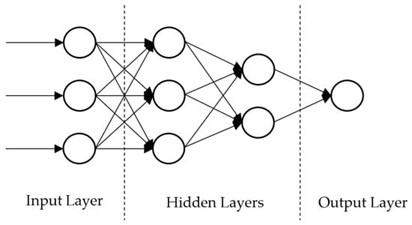
\includegraphics[width=0.8\textwidth, center]{images/Picture1.jpg}
    \caption{Struktur Neural Network}
    \label{fig:neural-network} 
\end{afigure}

\subsection{Fungsi Aktivasi}
Fungsi aktivasi adalah sebuah persamaan matematika yang tujuannya untuk mengaktifkan node yang ada di jaringan saraf. Node yang aktif akan menghasilkan keluaran sesuai dengan jenis fungsi aktivasi. Terdapat beberapa jenis fungsi aktivasi yang dapat digunakan sesuai dengan kebutuhan. Fungsi aktivasi yang umum digunakan dalam proses klasifikasi adalah fungsi aktivasi \textit{Rectified Linear Unit} (ReLu) dan juga fungsi aktivasi softmax. Berikut merupakan penjelasan lebih lanjut dari fungsi aktivasi tersebut:

\begin{enumerate}
    \item \textbf{\textit{Rectified Linear Unit}}
    \item[] \textit{Rectified Linear Unit} (ReLu) merupakan sebuah fungsi aktivasi yang sering digunakan pada pembuatan model \textit{machine learning}. Fungsi ReLu sering digunakan pada lapisan-lapisan tersembunyi (\textit{hidden layers}) karena kesederhanaan komputasi yang dilakukan oleh fungsi ini. Hal ini dikarenakan tidak adanya komputasi yang terlalu rumit sehingga membuat proses pelatihan suatu model dapat dijalankan dalam waktu yang relatif singkat.
    
    ReLu menggunakan fungsi f(z) = max(0, z), yang artinya jika output positif maka akan menghasilkan nilai yang sama, jika tidak maka akan menghasilkan nilai 0. ReLu tidak hanya meningkatkan kinerja secara signifikan tetapi juga membantu mengurangi jumlah perhitungan selama fase pelatihan. Hal ini terjadi akibat dari nilai 0 dalam output ketika nilai z negatif, sehingga menonaktifkan neuron \cite{moolayil2019}.
    \begin{afigure}
        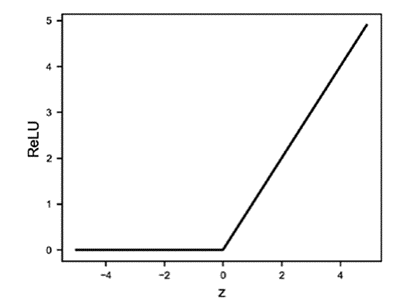
\includegraphics[width=0.8\textwidth, center]{images/Picture2.png}
        \caption{Grafik Fungsi Aktivasi ReLu}
        \label{fig:relu} 
    \end{afigure}

    \item \textbf{\textit{Softmax}}
    \item[] \textit{Softmax} merupakan fungsi aktivasi yang menginterpretasikan vektor nilai real X menjadi vektor nilai real sebagai probabilitas. Nilai probabilitas \textit{softmax} bergantung pada nilai recall yang dimasukkan ke dalam fungsi ini. Jika salah satu nilai input kecil atau negatif, nilai output dari fungsi \textit{softmax} adalah nilai probabilitas rendah. Nilai probabilitas tinggi diperoleh ketika fungsi ini menerima nilai masukan yang besar atau positif. Semua nilai output dari fungsi \textit{softmax} terletak antara 0 dan 1. 

    Fungsi \textit{softmax} sering digunakan dalam masalah klasifikasi dengan syarat kelas-kelas dalam data saling eksklusif. Hasil perhitungan MLP biasanya berupa titik-titik nyata, yang tidak mudah diskalakan dan sulit dimanipulasi. Fungsi \textit{softmax} mengubah titik-titik ini menjadi nilai probabilitas yang dinormalisasi, dan nilai probabilitas ini dapat digunakan sebagai input ke sistem lain. Ini adalah dasar untuk menggunakan fungsi aktivasi \textit{Softmax} di lapisan keluaran model pembelajaran mendalam seperti CNN. Definisi matematis dari \textit{softmax} sebagai persamaan 2.1 berikut:
    \begin{equation}
        \label{eq:softmax}
        \begin{split}
            S(x)_i = \frac{e^{x_i}}{\sum_{j=1}^{n} e^{x_j}}
        \end{split}
    \end{equation}
    Dengan keterangan:
    \begin{itemize}
        \item \(x\) = Vektor input ke fungsi softmax, terdiri dari (x0, .... xK)
        \item \(x_i\)  = Elemen dari vektor input ke fungsi softmax, dan mereka dapat mengambil nilai real apa pun, positif, nol, atau negatif.
        \item \(e^{x_j}\) = Fungsi eksponensial standar diterapkan pada setiap elemen dari vektor input. Ini memberikan nilai positif di atas 0, yang akan sangat kecil jika inputnya negatif, dan sangat besar jika inputnya besar. Namun, itu masih belum ditetapkan dalam kisaran (0, 1) yang diperlukan dari suatu probabilitas.
        \item \({\sum_{j=1}^{n} e^{x_j}}\) Normalisasi. Normalisasi memastikan bahwa semua nilai keluaran fungsi akan berjumlah 1 dan masing-masing berada dalam kisaran (0, 1), sehingga merupakan distribusi probabilitas yang valid.
        \item n = Jumlah kelas dalam multi-class classifier.
        \item Nilai \(x_i\) adalah elemen dari vektor input dan dapat mengambil nilai ril.
    \end{itemize}
    Fungsi \textit{softmax} dinormalisasi seperti pada persamaan 2.1. Tujuannya adalah untuk memastikan bahwa semua nilai keluaran bersama-sama memiliki nilai 1, yang menunjukkan bahwa nilai ini adalah nilai probabilitas yang valid. \textit{Softmax} memperluas ide ini ke klasifikasi multi-kelas atau biasa disebut dengan klasifikasi multi-kelas. \textit{Softmax} memberikan nilai probabilitas untuk setiap kelas tugas klasifikasi. Nilai probabilitas total yang ditentukan harus 1, yang menunjukkan bahwa nilai tersebut merupakan nilai probabilitas yang valid.

\end{enumerate}

\subsection{\textit{Dropout}}
\textit{Dropout} merupakan teknik yang digunakan untuk menghindari \textit{overfitting} model. Dalam metode ini, aktivasi beberapa neuron yang dipilih secara acak dalam jaringan diasumsikan nol selama pelatihan. Neuron yang dipilih diubah di setiap iterasi pelatihan. Proses pembelajaran menjadi lebih andal dengan metode ini dan \textit{overfitting} berkurang.
\begin{afigure}
    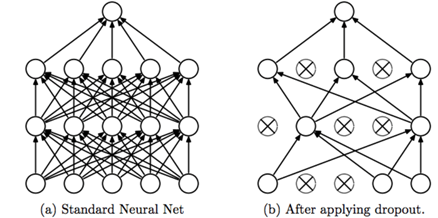
\includegraphics[width=0.8\textwidth, center]{images/Picture3.png}
    \caption{Neural Network Sebelum dan Sesudah Melakukan Dropout}
    \label{fig:dropout} 
\end{afigure}

Istilah \textit{dropout} mengacu pada pemutusan neuron (tersembunyi dan terlihat) dalam \textit{neural network}. Dengan mengeluarkan unit (neural) untuk sementara menghapusnya dari jaringan (\textit{network}), bersama dengan semua koneksi masuk dan keluarnya, seperti yang ditunjukkan pada Gambar 2.3. Pemilihan unit yang dijatuhkan secara acak \cite{yadav2022}. 


\subsection{\textit{Loss Function}}
\textit{Loss function}, atau disebut juga \textit{cost function}, adalah suatu fungsi matematis yang digunakan dalam \textit{machine learning} untuk mengukur seberapa baik model memetakan input ke output yang diharapkan. \textit{Loss function} menghitung selisih antara prediksi model dengan nilai \textit{ground truth}, atau nilai yang seharusnya dihasilkan oleh model.

Tujuan dari \textit{loss function} adalah untuk mengoptimalkan model agar menghasilkan prediksi yang semakin mendekati nilai \textit{ground truth}. Untuk itu, \textit{loss function} sering digunakan sebagai acuan dalam proses optimasi, di mana model akan mencoba meminimalkan nilai \textit{loss function} tersebut dengan menyesuaikan parameter model. Contoh umum dari \textit{loss function} adalah \textit{Mean Squared Error} (MSE), \textit{cross-entropy loss}, dan \textit{hinge loss}. Pemilihan \textit{loss function} yang tepat sangat penting dalam pengembangan model, tergantung pada jenis masalah dan tipe data yang digunakan.

\section{Dataset}
Dataset merupakan istilah yang merujuk pada kumpulan data. Dataset berisi lebih dari satu variabel dan menyangkut suatu topik tertentu. Dataset adalah representasi di memori dari satu tabel atau lebih dan digunakan untuk menyimpan baris yang didapatkan saat permintaam dikirim ke basis data. dataset dapat ditambahkan, dihapus, atau diperbarui.

Dataset tetap ada di memori dan data didalamnya bisa dimanipulasi dan diperbarui tanpa bergantung pada asalnya. Jika diperlukan, dataset bisa bertindak sebagai template untuk memperbarui data pusat. Dataset dapat dibagi menjadi data training dan data testing. Data training digunakan untuk melatih algoritma dalam mencari model yang sesuai sedangkan data testing akan dipakai untuk menguji dan mengetahui performa model yang didapatkan pada tahap testing.

\section{\textit{Epoch}}
\textit{Epoch} adalah ketika seluruh dataset sudah melalui proses training pada Neural Network sampai dikembalikan ke awal untuk sekali putaran, karena satu \textit{epoch} terlalu besar untuk dimasukkan kedalam komputer maka dari itu perlu membaginya kedalam satuan kecil. \textit{Epoch} digunakan untuk mengoptimalkan pembelajaran dan grafik yang digunakan.

Seiring bertambahnya jumlah \textit{epoch}, semakin banyak pula bobot yang berubah dalam neural network. Jumlah \textit{epoch} yang digunakan tidak ditentukan, jumlah epoch yang digunakan terkait dengan beragamnya data yang digunakan atau tergantung dengan dataset yang dimiliki.

\section{Citra}
Citra merupakan suatu gambaran atau kemiripan dari suatu objek. Citra analog tidak dapat dipresentasikan dalam komputer, sehingga tidak bisa diproses oleh komputer secara langsung. Citra analog harus dikonversi menjadi citra yang dapat diolah oleh komputer sedangkan citra yang dihasilkan dari peralatan digital (Citra Digital) langsung bisa diolah oleh komputer. Citra di dalam peralatan digital terdapat sistem sampling dan kuantisasi sedangkan peralatan analog tidak dilengkapi kedua sistem tersebut. Sistem sampling adalah sistem yang mengubah citra kontinu menjadi Citra Digital dengan cara membagi Citra Analog menjadi M baris dan N kolom, sehingga menjadi citra diskrit. Semakin besar nilai M dan N, semakin halus citra digital yang dihasilkan. Pertemuan antara baris dan kolom disebut pixel. Sistem kuantisasi adalah Sistem yang melakukan pengubahan intensitas analog ke intensitas diskrit, sehingga dengan proses ini dimungkinkan untuk membuat gradasi warna sesuai dengan kebutuhan. Kedua sistem inilah yang bertugas untuk memotong-motong Citra menjadi M baris dan N kolom (proses sampling) sekaligus menentukan besar intensitas yang terdapat di titik tersebut (proses kuantisasi), sehingga menghasilkan resolusi Citra yang diinginkan \cite{andono2017}.

\section{Augmentasi Citra}
Augmentasi citra adalah sebuah teknik yang dapat menambahkan jumlah data latih dengan menghasilkan banyak varian yang realistis dari setiap contoh data latih \cite{geron2019}. Teknik ini dapat mengurangi kemungkinan permasalahan \textit{overfit} yang menjadikan teknik ini merupakan salah satu jenis teknik regularisasi. Data citra hasil augmentasi harus serealistis mungkin sehingga manusia tidak dapat membedakan data hasil augmentasi dan data sebenarnya. Oleh karena itu, data artifisial dibuat dengan cara menggeser, memutar, dan mengubah ukuran dari setiap citra yang terdapat dalam data latih. Hasil dari proses pengubahan citra tersebut akan dimasukan ke dalam data latih.
\begin{afigure}
    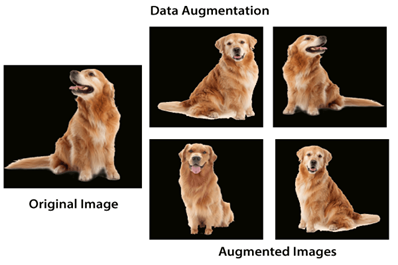
\includegraphics[width=0.8\textwidth, center]{images/Picture4.png}
    \caption{Hasil Teknik Augmentasi Citra}
    \label{fig:augmentasi-citra} 
\end{afigure}

Gambar 2.4 adalah contoh dari penggunaan teknik augmentasi citra. Hasil dari teknik ini menyerupai citra yang sesungguhnya. Teknik augmentasi citra biasa digunakan ketika dihadapkan dengan kondisi data yang sedikit dan sekiranya data tersebut kurang variasi. Data yang sedikit akan membuat model kurang mengenal variasi dari suatu citra sehingga model tersebut cenderung \textit{overfit}. Teknik augmentasi citra dapat membuat suatu model menambah pengetahuan mengenai fitur dari suatu citra dari hasil augmentasi citra. Semakin banyak fitur yang dipelajari dari sebuah citra, hal ini dapat meminimalisir kemungkinan model menjadi \textit{overfit}.

\section{Google}
Google adalah perusaham mesin pencari yang didirikan pada tahun 1998 oleh Sergey Brin dan Larry Page. Saat ini kantor utama Google ada di Mountain View, California. Lebih dari 70\% permintaan pencari online di seluruh dunia telah ditangani oleh Google.
Mesin pencari Google merupakan situs yang paling sukses dan popular. Banyaknya layanan dan produk online yang dapat digunakan seperti akun email. browser web. software produktivitas, ponsel dan aplikasi, alat pemetaan, \textit{e-book}, serta berbagai layanan lainnya membuat para penggunanya senang untuk menggunakan Google.

\subsection{Google Colaboratory}
Google Colaboratory lebih sering disebut sebagai "Google Colab" atau sekadar "Colab" adalah proyek penelitian untuk membuat prototipe model pembelajaran mesin pada opsi perangkat keras canggih seperti GPU dan TPU. Ini menyediakan lingkungan notebook Jupyter tanpa server untuk pengembangan interaktif. Google Colab gratis untuk digunakan seperti produk Google lainnya \cite{bisong2019}.
\begin{afigure}
    
\includegraphics[width=0.8\textwidth, center]{images/Picture5.png}
    \caption{Google Colaboratory}
    \label{fig:google-colab} 
\end{afigure}
Google Colab atau Colaboratory adalah layanan cloud gratis yang dihosting oleh Google untuk mendorong penelitian \textit{Machine Learning} dan \textit{Artificial Intelligence}, yang sering kali menjadi penghalang pembelajaran dan kesuksesan adalah persyaratan kekuatan komputasi yang sangat besar \cite{naik2023}.

\section{Python}
Code Python adalah bahasa pemrograman interpretatif yang bisa dipasang pada berbagai platform, khususnya platform yang berfokus pada keterbacaan kode. Kode Python bisa di-embed ke bahasa lain seperti C dan Java, atau sebaliknya, dari bahasa C atau Java ke Python. Pemrograman Python itu merupakan salah satu bahasa pemrograman yang dapat melakukan eksekusi sejumlah instruksi multu guna secara langsung dengan metode Object Oriented Programming dan menggunakan semantik dinamis untuk memberikan tingkat keterbacaan sintak. 

Pemrograman Python memiliki bahsa yang kemampuan, menggabungkan kapabilitas dan sintaksis kode yang jelas dan dilengkapi dengan fungsionalitas pustaka standar yang besar serta komprehensif. Pemrograman Bahasa Python difokuskan untuk digunakan dalam menganalisis data, visualisasi data, membuat dan mengembangkan AI. Pemrograman Python adalah pemrograman yang paling mudah di pelajari dengan code yang pendek dan tidak susah. Python memiliki pustaka (\textit{library}) yang luas dan dapat dikembangkan ke bidang-bidang lainnya. Beberapa \textit{library} python yang popular dalam Data Science dan AI adalah Scikit-Learn, TensorFlow,PyTorch. 

Pemrograman bahasa Python merupakan bahasa pemrograman yang tidak menggunakan compiler. Dengan sifat open-source yang dimilikinya, pengguna dapat mempelajari Python dengan mudah karena bahasa ini dapat dugunakan dalam membuat situs,mengembangkan situs, mengembangkan video game, membangun GUI Desktop, dan mengembangkan perangkat lunak \cite{setiawan2022}.

\section{Tensorflow}
TensorFlow adalah salah satu pustaka deep learning yang paling populer, yang awalnya dikembangkan oleh peneliti di Google. TensorFlow sangat memudahkan dan mempercepat penelitian dan penerapan model jaringan saraf. Pustaka ini mencakup konsep-konsep inti seperti fungsi konstruksi graf, alat eksekusi graf, dan alat visualisasi TensorBoard \cite{bopang2020}.

TensorFlow adalah sebuah platform open source untuk \textit{machine learning} yang dibuat oleh Google. TensorFlow memungkinkan pengembang dan peneliti untuk membuat dan melatih model \textit{machine learning} dari berbagai jenis data, seperti gambar, teks, dan suara. TensorFlow menggunakan konsep tensor, yaitu struktur data multidimensi, sebagai representasi dari data masukan dan keluaran dalam model \textit{machine learning}. TensorFlow menyediakan banyak pustaka dan algoritma \textit{machine learning} yang dapat digunakan untuk membangun berbagai jenis model, seperti \textit{neural network}, \textit{decision tree}, dan \textit{regression model}. TensorFlow memiliki fitur yang kuat untuk distribusi dan skalabilitas, sehingga dapat digunakan untuk menangani data yang sangat besar dan kompleks. TensorFlow juga mendukung berbagai platform, termasuk \textit{desktop}, \textit{server}, dan perangkat \textit{mobile}.
    
Salah satu kelebihan TensorFlow adalah mudahnya penggunaannya, terutama untuk pengguna Python, karena TensorFlow menyediakan API yang mudah digunakan dan dokumentasi yang lengkap. Selain itu, TensorFlow juga memiliki komunitas yang besar dan aktif, sehingga pengguna dapat dengan mudah menemukan sumber daya dan dukungan dalam pengembangan model \textit{machine learning} mereka.

\section{Keras}
Keras adalah antarmuka pemrograman aplikasi (API) berbasis Python yang dirancang untuk mempermudah pembuatan dan pelatihan model jaringan saraf. Keras dikembangkan untuk berjalan di atas kerangka pembelajaran mesin seperti TensorFlow, Theano, atau CNTK. Keras menekankan kemudahan penggunaan dan modularitas, memungkinkan pengguna untuk membangun dan menguji model \textit{deep learning} dengan cepat dan efisien \cite{chicho2021}.

Keras merupakan sebuah pustaka open source untuk \textit{machine learning} yang dibangun di atas bahasa pemrograman Python. Keras menyediakan antarmuka tingkat tinggi untuk membangun dan melatih model \textit{machine learning} dengan mudah dan cepat. Keras dirancang untuk memudahkan pembuatan model \textit{neural network} dengan menyediakan API yang sederhana dan intuitif. Keras mendukung berbagai jenis model \textit{neural network}, termasuk model \textit{feedforward}, model \textit{recurrent}, dan model \textit{convolutional}.  

Salah satu kelebihan Keras adalah fleksibilitasnya dalam menggunakan \textit{backend} untuk komputasi numerik. Keras dapat digunakan dengan beberapa \textit{backend}, termasuk TensorFlow, Theano, dan Microsoft Cognitive Toolkit. Keras juga menyediakan berbagai algoritma \textit{machine learning} yang siap digunakan, termasuk optimasi, regularisasi, dan fungsi aktivasi. Selain itu, Keras juga menyediakan berbagai utilitas untuk memproses data dan mengelola model, seperti operasi matriks dan fungsi pembagian data.

Keras telah menjadi salah satu pustaka \textit{machine learning} paling populer di dunia, karena mudah digunakan, cepat, dan fleksibel. Keras juga memiliki komunitas yang besar dan aktif, sehingga pengguna dapat dengan mudah menemukan sumber daya dan dukungan dalam pengembangan model \textit{machine learning} mereka. Sekarang, Keras telah diintegrasikan ke dalam TensorFlow sebagai bagian dari proyek TensorFlow.

\section{Scikit-learn}
Scikit-learn merupakan sebuah \textit{library open-source} yang digunakan untuk \textit{machine learning} pada bahasa pemrograman Python. \textit{Library} ini menyediakan berbagai algoritma \textit{machine learning}, seperti klasifikasi, regresi, pengelompokan, dan pengurutan data. Selain itu, scikit-learn juga dilengkapi dengan berbagai fitur untuk memproses dan memanipulasi data, seperti \textit{preprocessing}, \textit{feature selection}, dan \textit{data transformation}.

Scikit-learn atau sklearn merupakan sebuah module dari bahasa pemrograman Python yang dibangun berdasarkan NumPy, SciPy, dan Matplotlib. Fungsi dari module ini adalah untuk membantu melakukan processing data ataupun melakukan training data untuk kebutuhan machine learning atau data science. Banyak sekali fitur yang ada pada module ini seperti model – model klasifikasi, \textit{clustering}, regresi berbasis model machine learning dan proses – proses yang dapat dimanfaatkan pada tahap \textit{Feature Engineering} seperti reduksi dimensi menggunakan PCA. Module ini sangatlah popular dan sering digunakan dikalangan \textit{data scientist} karena banyak sekali model – model \textit{machine learning} yang dapat kita panggil menggunakan module ini \cite{bisaai2024scikit}.

Scikit-learn dirancang untuk menjadi mudah digunakan dan dapat diakses oleh pengguna dengan berbagai tingkat keahlian dalam machine learning. Library ini memiliki dokumentasi yang lengkap dan tutorial yang tersedia di website resminya sehingga memudahkan pengguna untuk mempelajari dan mengimplementasikan algoritma machine learning. Beberapa fitur dari scikit-learn antara lain:
\begin{enumerate}
    \item \textbf{Algoritma \textit{machine learning} yang lengkap}
    \item[] Scikit-learn menyediakan beragam algoritma machine learning, mulai dari algoritma yang sederhana hingga yang kompleks, seperti \textit{Decision Tree}, \textit{Random Forest}, \textit{Naive Bayes}, \textit{Support Vector Machine}, dan \textit{Neural Network}.
    \item \textbf{\textit{Preprocessing Data}}
    \item [] Scikit-learn dilengkapi dengan berbagai fitur untuk memproses dan memanipulasi data, seperti \textit{handling missing values}, \textit{scaling data}, \textit{encoding} kategorikal data, dan lain-lain.
    \item \textbf{\textit{Feature Selection}}
    \item[] Scikit-learn menyediakan berbagai teknik untuk memilih fitur yang paling relevan dalam dataset, seperti SelectKBest, \textit{Principal Component Analysis} (PCA), dan \textit{Recursive Feature Elimination} (RFE).
    \item \textbf{Evaluasi Model}
    \item[] Scikit-learn memiliki berbagai metrik evaluasi untuk mengukur performa model, seperti \textit{accuracy}, \textit{precision}, \textit{recall}, \textit{F-1 Score}, dan lain-lain. 
\end{enumerate}

Scikit-learn telah digunakan dalam berbagai aplikasi dalam bidang \textit{machine learning}, seperti klasifikasi spam email, prediksi harga saham, deteksi penyakit, dan lain-lain. \textit{Library} ini juga dapat digunakan bersamaan dengan \textit{library} Python lainnya, seperti NumPy, Pandas, dan Matplotlib untuk memproses dan memvisualisasikan data secara efektif.

\section{Adam \textit{Optimizer}}
\textit{Optimizer} adalah metode atau algoritma yang digunakan untuk memecahkan masalah optimisasi dalam \textit{machine learning}. Tujuan utamanya adalah untuk menemukan parameter model yang meminimalkan atau memaksimalkan fungsi objektif. \textit{Optimizer} berperan penting dalam proses pembelajaran mesin, di mana esensi dari sebagian besar algoritma \textit{machine learning} adalah membangun model optimisasi dan mempelajari parameter dalam fungsi objektif dari data yang diberikan \cite{sun2019}.

\textit{Optimizer} adalah sebuah algortima yang berfungsi untuk meminimalkan fungsi kesalahan atau untuk memaksimalkan efisiensi produksi. \textit{Optimizer} biasanya berupa fungsi matematika yang bergantung pada parameter model yang dapat dipelajari seberti bobot dan bias. \textit{Optimizer} dapat membantu proses pelatihan suatu model \textit{deep learning} dengan cara mengubah bobot dan bias untuk mengurangi kerugian.

Adam \textit{optimizer} adalah algoritma optimasi yang sering digunakan dalam \textit{machine learning} untuk mengoptimalkan model \textit{neural network}. Adam merupakan singkatan dari "\textit{adaptive moment estimation}", yang merujuk pada kemampuan algoritma ini untuk menyesuaikan laju pembelajaran (\textit{learning rate}) untuk setiap parameter dalam model secara adaptif.

Adam \textit{optimizer} adalah algoritma optimasi yang banyak digunakan dalam pelatihan jaringan saraf dalam. Algoritma ini menggabungkan keuntungan dari dua metode optimasi sebelumnya, yaitu AdaGrad dan RMSProp, dengan melacak rata-rata momentum pertama (mean) dan kedua (variance) dari gradien. Adam mengadaptasi laju pembelajaran untuk setiap parameter, membuatnya sangat efektif dalam mengatasi masalah gradien yang jarang \cite{bock2019}.

Secara umum, Adam \textit{optimizer} memperhitungkan gradien dari seluruh data latih saat memperbarui parameter, dan menghitung laju pembelajaran adaptif untuk setiap parameter dalam model. Hal ini memungkinkan Adam \textit{optimizer} untuk menyesuaikan laju pembelajaran secara adaptif untuk setiap parameter, tergantung pada kondisi lokal dari gradien.

Adam \textit{optimizer} telah terbukti efektif dalam mempercepat konvergensi dalam pelatihan model \textit{neural network}, terutama pada masalah yang kompleks dan data yang besar. Selain itu, Adam \textit{optimizer} juga mudah diimplementasikan dan digunakan dalam berbagai jenis model \textit{neural network}.

\section{\textit{Transfer Learning}}
\textit{Transfer learning} merupakan sebuah teknik yang memanfaatkan representasi fitur dari model yang telah dilatih sebelumnya sehingga saat melatih model baru, tidak perlu melatih model tersebut dari awal. Model pra-pelatihan umumnya dilatih pada dataset yang besar yang menjadi patokan standar dalam bidang visi komputer. Bobot yang dihasilkan dari model yang telah dilatih dapat diterapkan pada model baru untuk menyelesaikan masalah visi komputer dan lainnya. Model pra-pelatihan dapat langsung digunakan dalam membuat prediksi tugas baru atau diintegrasikan ke dalam pelatihan model baru. Penggunaan model pra-pelatihan dalam model baru dapat menghasilkan waktu pelatihan yang lebih cepat dan kesalahan generalisasi yang lebih rendah. \textit{Transfer learning} sangat bermanfaat ketika data pelatihan terbatas. Bobot yang terdapat pada model pra-pelatihan dapat digunakan untuk memprediksi fitur-fitur pada data latih sehingga pelatihan dapat dilakukan dalam waktu yang lebih singkat \cite{zhuang2020}. Terdapat 5 tahap dalam implementasi transfer learning, yaitu:
\begin{enumerate}
    \item \textbf{Menentukan model pra-pelatihan}
    \item[] Langkah pertama adalah menentukan model pra-pelatihan yang ingin digunakan. Pemilihan model pra-pelatihan dapat dilakukan dengan cara melihat performa model tersebut pada dataset yang besar.
    \item \textbf{Membuat model dasar}
    \item [] Proses ini dilakukan dengan cara mengimplementasikan arsitektur dari model pra-pelatihan seperti EfficientNetV2. Proses ini dilakukan dengan cara mengunduh bobot pra-pelatihan secara opsional, hal ini dilakukan agar model dasar yang dibuat memiliki dasar pengetahuan untuk kasus tertentu. Pada umumnya model dasar akan memiliki lebih banyak unit di lapisan keluaran akhir daripada yang dibutuhkan. Saat membuat model dasar, diharuskan untuk menghapus lapisan keluaran akhir. Selanjutnya adalah menambahkan lapisan keluaran akhir yang kompatibel dengan masalah tertentu.
    \item \textbf{\textit{Freezing Layer}}
    \item[] \textit{Freezing layer} dilakukan pada model dasar. Hal ini bertujuan agar bobot pada lapisan model dasar tidak diinisialisasi ulang pada saar proses pelatihan. Jika tidak melakukan \textit{freezing layer}, maka beban yang sebelumnya telah diunduh akan hilang secara keseluruhan dan pelatihan model dilakukan dari awal yang dapat memakan waktu lebih lama.
    \item \textbf{Melatih layer baru untuk dataset baru}
    \item[] Layer baru adalah layer yang dibuat untuk menyesuaikan layer output dengan dataset baru tanpa mengubah layer yang telah dibekukan (\textit{freeze}) sebelumnya. Hal ini dilakukan karena layer output dari model pra-pelatihan umumnya telah disesuaikan dengan kebutuhan dataset besar yang dilatih sebelumnya, seperti ImageNet yang memiliki 1000 kelas. Tentu ini tidak selalu relevan dengan dataset baru yang digunakan, sebagai contoh apabila dataset yang digunakan untuk melatih model baru hanya memiliki 2 kelas, maka layer output ini tidak sesuai. Oleh karena itu layer output harus disesuaikan dengan kebutuhan dataset baru.
    \item \textbf{Meningkatkan performa model dengan \textit{fine-tuning}}
    \item[] Performa suatu model \textit{machine learning} tentu tidaklah selalu baik untuk semua tipe dataset. Hal ini juga yang dapat menyebabkan model pra-pelatihan kurang cocok digunakan untuk suatu tipe dataset tertentu. \textit{Fine-tuning} adalah sebuah metode untuk mengubah parameter yang ada pada model tertentu pada saat proses pelatihan dan melakukan proses pelatihan ulang. Salah satu parameter yang berpengaruh pada saat proses pelatihan adalah \textit{learning rate}. Pemilihan nilai \textit{learning rate} yang tepat akan membuat performa model meningkat dan dapat memprediksi tugas sesuai yang diinginkan.
\end{enumerate}

\section{\textit{Convolutional Neural Network}}
\textit{Convolutional Neural Network} atau dapat disingkat dengan CNN merupakan salah satu jenis deep learning. \textit{Machine learning} memiliki cabang yaitu \textit{deep learning} yang berguna untuk membuat komputer dapat melakukan pekerjaan seperti pekerjaan manusia. \textit{Convolutional Neural Network} bekerja dengan meniru berkomunikasi dengan neuron yang cara kerja dari saraf-saraf manusia berhubungan.

Sebagai algoritma dengan kinerja yang sangat baik, CNN telah banyak digunakan di bidang pemrosesan citra dan mencapai hasil yang baik dengan mengandalkan bidang reseptif lokalnya sendiri, pembagian bobot, penggabungan, dan koneksi yang terpisah \cite{tian2020}.

\begin{afigure}
    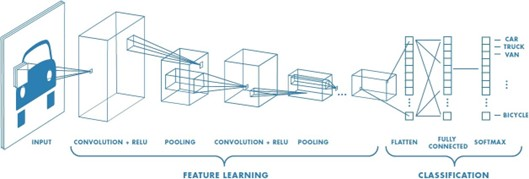
\includegraphics[width=0.9\textwidth, center]{images/Picture6.jpg}
    \caption{Arsitektur Convolutional Neural Network (CNN)}
    \label{fig:cnn} 
\end{afigure}

Pada Gambar 2.6, tahap pertama pada arsitektur\textit{ Convolutional Neural Network} yaitu tahap Konvolusi, kemudian dilanjutkan menuju fungsi aktivasi yang biasanya menggunakan fungsi aktivitas \textit{Rectifier Linear Unit} atau ReLU. Proses \textit{Pooling} merupakan proses setelah fungsi aktivasi yang dimana proses ini diulang beberapa kali sampai mendapatkan peta fitur agar dapat melanjutkan ke \textit{fully connected neural network}.

Setelah \textit{fully connected neural network} akan dilanjutkan ke \textit{output class}. \textit{Convolutional layer} merupakan bagian dari tahap pada arsitektur CNN. Tahap ini melakukan operasi konvolusi pada output dari layer sebelumnya. Layer tersebut merupakan proses utama yang mendasari jaringan arsitektur CNN. Konvolusi merupakan istilah matematis dimana pengaplikasian sebuah fungsi pada output fungsi lain secara berulang. Operasi konvolusi merupakan operasi pada 2 fungsi argumen bernilai nyata. Operasi ini menerapkan fungsi output sebagai feature map dari input citra. Input dan output ini dapat dilihat sebagai 2 argumen bemilai real.

\section{Lapisan \textit{Convolutional Neural Network} (CNN)}
\textit{Convolutional Neural Network} (CNN) terdiri atas tiga lapis (layer) yaitu \textit{input layer}, \textit{output layer}, dan beberapa \textit{hidden layers}. \textit{Hidden layer} umumnya berisi \textit{convolutional layers},\textit{ pooling layers}, \textit{normalization layers}, ReLu layer, \textit{fully connected layers}, dan serta \textit{loss layer} \cite{alom2018}.

\subsection{\textit{Convolutional Layer}}
Lapisan konvolusi, atau \textit{Convolutional Layer}, merupakan komponen utama dalam jaringan saraf konvolusional (CNN) yang berfungsi untuk mengekstraksi fitur-fitur dari input citra. Lapisan ini menggunakan filter atau kernel yang bergerak melintasi citra untuk melakukan operasi konvolusi, menghasilkan peta fitur (\textit{feature map}) sebagai output. Setiap filter dalam lapisan ini belajar mendeteksi pola-pola spesifik, seperti tepi, tekstur, atau warna, dengan menerapkan bobot tertentu pada piksel dalam citra input. Hasil dari operasi konvolusi ini membantu jaringan dalam mengenali dan memahami elemen-elemen penting dari citra yang diolah. Dengan demikian, lapisan konvolusi adalah kunci dalam mengubah data citra mentah menjadi representasi fitur yang dapat digunakan oleh lapisan-lapisan berikutnya dalam jaringan untuk tugas-tugas seperti klasifikasi dan deteksi objek \cite{Goodfellow-et-al-2016}.

\subsection{\textit{Activation Layer}}
Lapisan aktivasi, atau \textit{Activation Layer}, adalah bagian penting dari jaringan saraf konvolusional (CNN) yang memperkenalkan non-linearitas ke dalam model. Setelah operasi konvolusi menghasilkan peta fitur, lapisan ini menerapkan fungsi aktivasi seperti ReLU (Rectified Linear Unit) yang mengubah semua nilai negatif menjadi nol dan mempertahankan nilai positif. Fungsi aktivasi lainnya yang sering digunakan termasuk Sigmoid dan Tanh, meskipun ReLU lebih umum dalam CNN karena sifatnya yang mempercepat konvergensi. Dengan menambahkan non-linearitas, lapisan aktivasi memungkinkan model untuk belajar dari data yang lebih kompleks dan meningkatkan kemampuannya dalam menyelesaikan masalah klasifikasi dan deteksi objek \cite{Goodfellow-et-al-2016}.

\subsection{\textit{Pooling Layer}}
Lapisan \textit{pooling}, atau \textit{Pooling Layer}, digunakan untuk mengurangi dimensi spasial dari peta fitur yang dihasilkan oleh lapisan konvolusi, yang membantu mengurangi jumlah parameter dan komputasi dalam jaringan. Dua jenis pooling yang umum digunakan adalah \textit{Max Pooling} dan \textit{Average Pooling}. \textit{Max Pooling} mengambil nilai maksimum dari setiap patch kecil peta fitur, sementara \textit{Average Pooling} mengambil rata-rata nilai. Proses \textit{pooling} membantu membuat representasi fitur lebih tahan terhadap pergeseran dan distorsi kecil dalam gambar, sehingga meningkatkan ketahanan model terhadap variasi pada data input \cite{Goodfellow-et-al-2016}.
\begin{enumerate}
        \item \textbf{\textit{Max Pooling}}
        \item[] \textit{Max pooling} merupakan metode \textit{pooling} yang paling populer. Operasi ini dilakukan dengan cara mengambil neuron dengan nilai aktivasi tertinggi di setiap bidang reseptif lokal (\textit{grid cell}), dan hanya mengambil nilai tertinggi dan mengirim nilai itu ke proses selanjutnya. Pada Gambar 2.7 merupakan contoh max pooling, dimana bidang yang berjumlah 4x4, diperkecil menjadi bidang reseptif 2x2 dengan cara mengambil nilai yang terbesar \cite{vasilev2019}.
        \begin{afigure}
            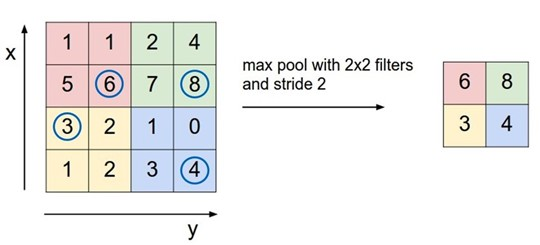
\includegraphics[width=0.8\textwidth, center]{images/Picture7.jpg}
            \caption{Proses Max Pooling}
            \label{fig:max-pooling} 
        \end{afigure}
        \item \textbf{\textit{Average Pooling}}
        \item[] \textit{Average pooling} merupakan metode \textit{pooling} lainnya, di mana output dari masing-masing bidang reseptif adalah nilai rata-rata dari semua aktivasi dalam bidang tersebut. Pada Gambar 2.8 merupakan contoh \textit{average pooling} dengan cara mengambil nilai rata-rata untuk memperkecil ukuran \cite{vasilev2019}.
        \begin{afigure}
            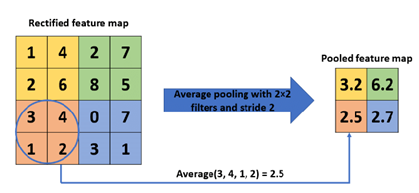
\includegraphics[width=0.8\textwidth, center]{images/Picture8.png}
            \caption{Proses Average Pooling}
            \label{fig:avg-pooling} 
        \end{afigure}
    \end{enumerate}

\subsection{\textit{Fully Connected Layer}}
Lapisan fully connected, atau \textit{Fully Connected Layer}, biasanya ditempatkan di bagian akhir CNN, di mana setiap neuron terhubung dengan semua neuron di lapisan sebelumnya. Lapisan ini berfungsi untuk menggabungkan fitur-fitur yang diekstraksi oleh lapisan konvolusi dan \textit{pooling} untuk melakukan klasifikasi akhir. Data yang diterima oleh lapisan ini diubah menjadi satu dimensi dan kemudian diproses oleh sejumlah neuron yang dapat memprediksi kelas dari input. Lapisan \textit{fully connected} ini sering kali diikuti oleh fungsi aktivasi seperti Softmax (untuk masalah klasifikasi multi-kelas) atau Sigmoid (untuk masalah klasifikasi biner) untuk menghasilkan probabilitas dari kelas-kelas yang diprediksi \cite{Goodfellow-et-al-2016}.

\subsection{\textit{Normalization Layer}}
Lapisan normalisasi, atau \textit{Normalization Layer}, seperti Batch Normalization, digunakan untuk menormalkan input dari satu lapisan sebelum memasuki lapisan berikutnya. Normalisasi dilakukan dengan cara menstandarkan aktivasi dari layer sebelumnya untuk setiap \textit{mini-batch}, dengan mempertahankan rata-rata dan variansi tertentu. Proses ini membantu dalam mempercepat proses pelatihan dan membuat model lebih stabil dengan mengurangi masalah \textit{vanishing gradients} dan\textit{ exploding gradients}, yang umum terjadi dalam jaringan saraf yang dalam \cite{ioffe2015}.

\subsection{\textit{Output Layer}}
Lapisan output, atau \textit{Output Layer}, adalah lapisan terakhir dalam CNN yang memberikan hasil akhir dari jaringan. Untuk masalah klasifikasi, lapisan ini biasanya terdiri dari neuron sebanyak jumlah kelas yang ada dalam data dan menggunakan fungsi aktivasi seperti Softmax untuk mengubah skor menjadi probabilitas. Probabilitas ini kemudian digunakan untuk menentukan kelas dari input citra. Fungsi aktivasi Softmax membantu dalam menghasilkan distribusi probabilitas dari berbagai kelas, sehingga memudahkan dalam penentuan keputusan akhir \cite{Goodfellow-et-al-2016}.

\section{EfficientNet}
EfficientNet merupakan arsitektur \textit{Convolutional Neural Network} atau CNN dan metode penskalaan yang secara seragam menskala semua dimensi kedalaman (\textit{depth}), lebar (\textit{width}), dan resolusi menggunakan koefisien gabungan (\textit{compound coefficient}). Metode penskalaan EfficientNet didasarkan pada intuisi bahwa jika gambar input lebih besar, maka jaringan membutuhkan lebih banyak lapisan untuk meningkatkan bidang reseptif (\textit{receptive field}) dan lebih banyak saluran untuk menangkap pola yang lebih detail pada gambar yang lebih besar. 

EfficientNet telah menunjukkan performa yang sangat baik dalam berbagai tugas \textit{transfer learning}, mencapai akurasi \textit{state-of-the-art} pada dataset seperti CIFAR-100 (91,7\%), Flowers (98,8\%), dan tiga dataset \textit{transfer learning} lainnya, dengan jumlah parameter yang jauh lebih sedikit dibandingkan model-model sebelumnya \cite{tan2020}. 

\subsection{EfficientNetV2}
Model EfficientNetV2 merupakan keluarga baru dari \textit{Convolutional Neural Network} (CNN) yang memiliki kemampuan unggul dalam pengklasifikasian gambar, karena mampu 11x lebih cepat dalam pelatihan dan model yang 6.8x lebih kecil. EfficientNetV2 menggunakan blok \textit{Mobile Inverted Bottleneck Convolution} (MBConv) dengan rasio ekspansi yang lebih kecil dan Fused-MBConv yang ditambahkan pada lapisan awal serta menggunakan kernel berukuran 3x3 yang lebih kecil dengan beberapa layer \cite{tan2021}.
\begin{afigure}
    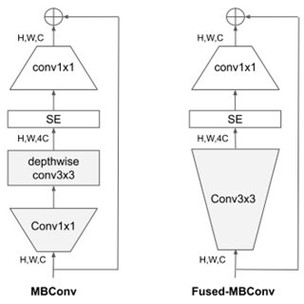
\includegraphics[width=0.6\textwidth, center]{images/Picture9.jpg}
    \caption{Struktur MBConv dan Fused-MBConv}
    \label{fig:mbconv} 
\end{afigure}

Gambar 2.9 menunjukkan struktur dari MBConv dan Fused- MBConv. Blok Mobile Inverted Bottleneck Convolution (MBConv) dan Fused-MBConv pada EfficientNetV2 memiliki sedikit perbedaan layer yang digunakan. MBConv menggunakan depthwise conv3x3 dan Conv1x1, sedangkan Fused-MBConv menggunakan Conv3x3.

\begin{afigure}
    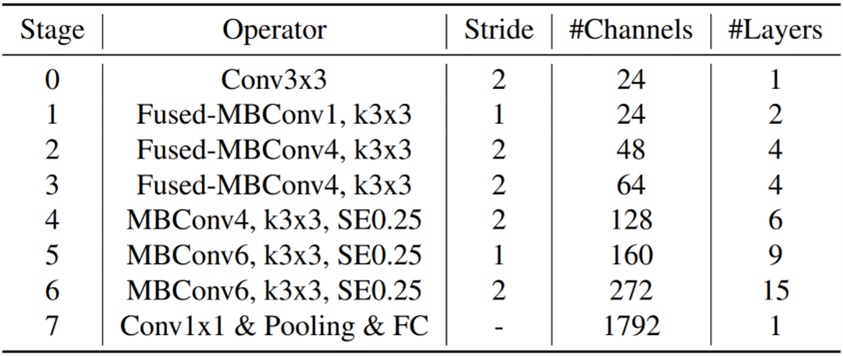
\includegraphics[width=0.6\textwidth, center]{images/Picture10.png}
    \caption{Arsitektur EfficientNetV2-S (Tan et al. 2021)}
    \label{fig:efficientnetv2} 
\end{afigure}

Gambar 2.10 menunjukkan blok-blok arsitektur EfficientNetV2-S. Blok-blok arsitektur EfficientNetV2 pada Gambar 2.10 terdiri dari layer Conv3x3 (layer konvolusi dengan kernel berukuran 3x3), Fused-MBConv k3x3 (kernel berukuran 3x3) dengan rasio ekspansi {1, dan 4}, MBConv k3x3 (kernel berukuran 3x3) dengan rasio ekspansi {4, dan 6}, dan Conv1x1 (layer konvolusi dengan kernel berukuran 1x1) \& Pooling \& FC layer. Total layer yang digunakan pada Gambar 2.10 berjumlah 42 layer.

\section{Grad-CAM}
\begin{afigure}
    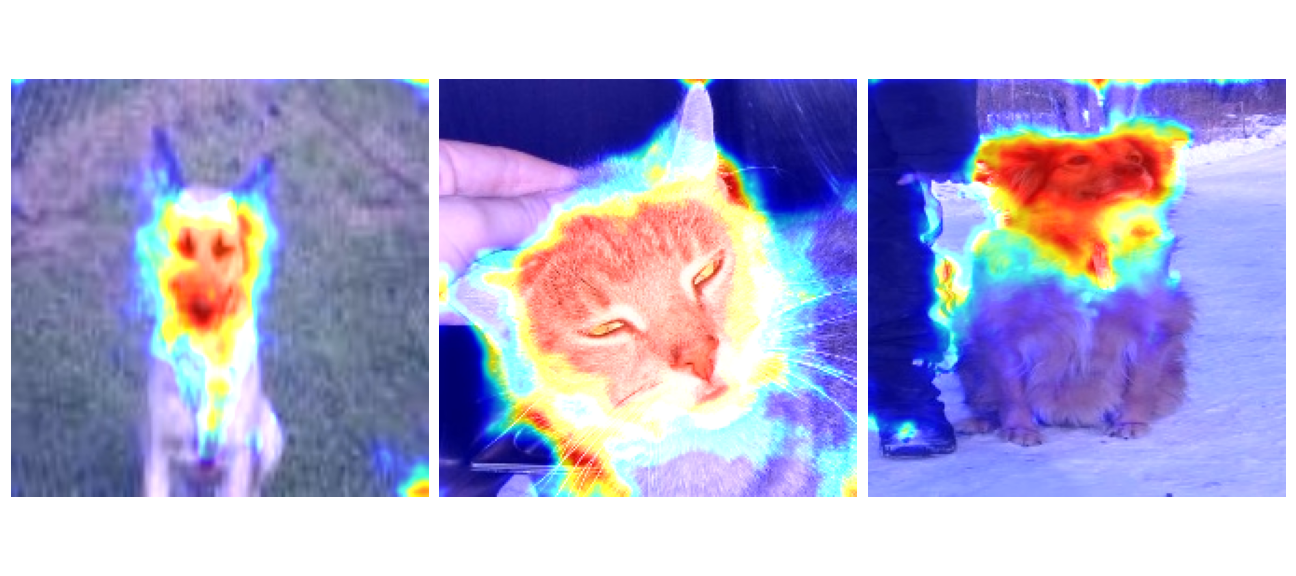
\includegraphics[width=0.9\textwidth, center]{images/Picture12.png}
    \caption{Contoh Visualisasi Grad-CAM}
    \label{fig:grad-cam} 
\end{afigure}
Grad-CAM atau \textit{Gradient-weighted Class Activation Mapping} merupakan teknik visualisasi yang menghasilkan penjelasan visual untuk keputusan yang dibuat oleh model \textit{Convolutional Neural Network}. Metode ini menggunakan gradien dari skor kelas target yang mengalir ke lapisan konvolusional terakhir untuk menghasilkan \textit{heatmap} yang menyoroti area penting dalam gambar yang mempengaruhi prediksi model. Grad-CAM merupakan generalisasi dari teknik \textit{Class Activation Mapping} (CAM), namun dapat diterapkan pada berbagai arsitektur CNN tanpa perlu memodifikasi atau melatih ulang model. Grad-CAM dapat digunakan untuk berbagai tugas seperti \textit{weakly-supervised localization}, segmentasi, dan memahami kegagalan serta bias model. Teknik ini membantu meningkatkan transparansi dan interpretabilitas model CNN dengan menunjukkan area mana dalam gambar yang paling berpengaruh terhadap keputusan klasifikasi \cite{selvaraju2017}.

\section{\textit{Flowchart}}
\begin{afigure}
    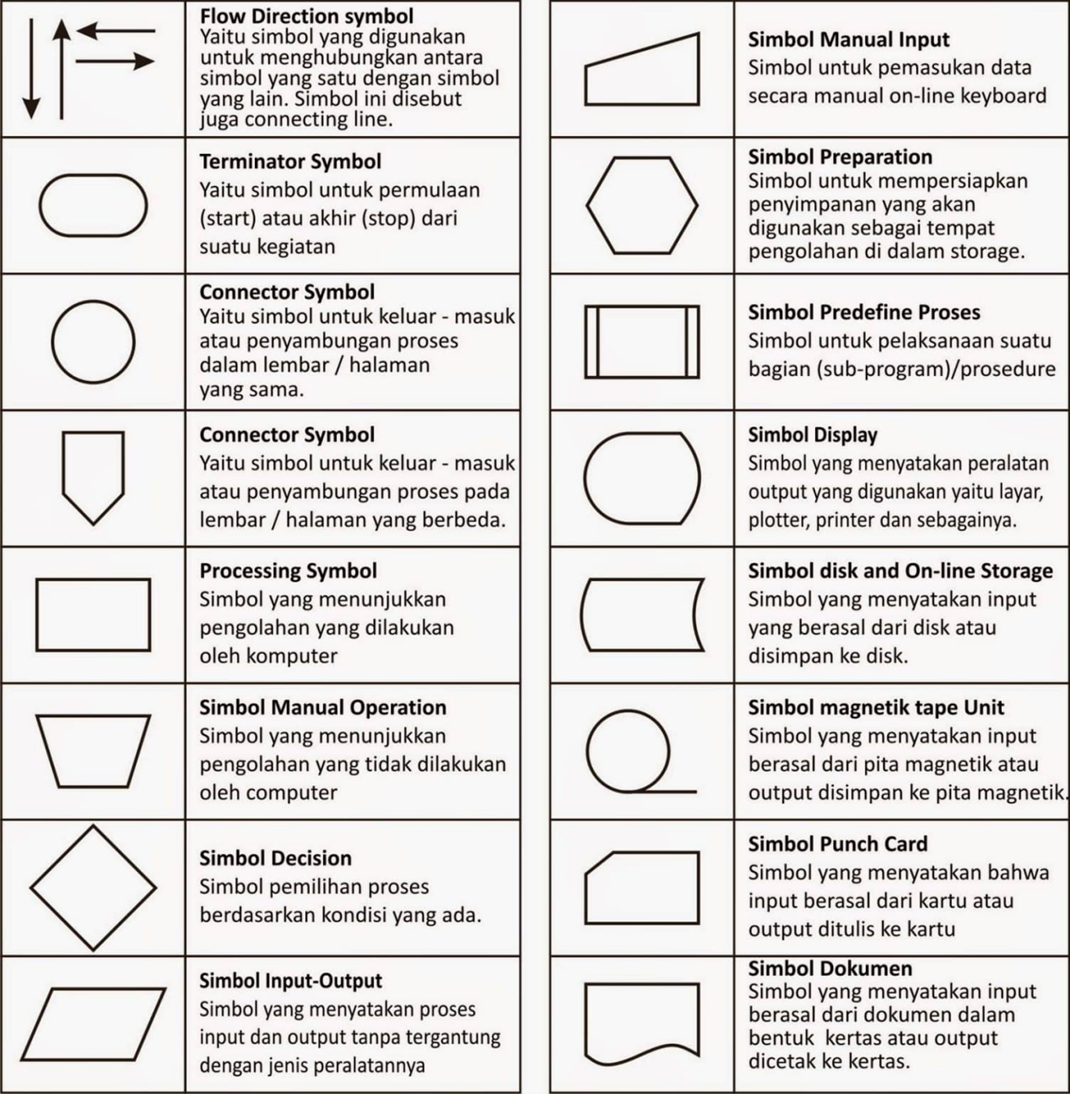
\includegraphics[width=0.85\textwidth, center]{images/Picture11.png}
    \caption{Simbol-Simbol Flowchart}
    \label{fig:flowchart} 
\end{afigure}
Menurut \cite{cmlabs2023},\textit{ Flowchart} adalah suatu bagan dengan simbol-simbol tertentu yang menggambarkan urutan proses secara mendetail dan hubungan antara suatu proses (instruksi) dengan proses lainnya dalam suatu program.
\textit{Flowchart} adalah suatu bagan dengan simbol-simbol tertentu yang menggambarkan urutan proses secara mendetail dan hubungan antara suatu proses (instruksi) dengan proses lainnya dalam suatu program. Pada perancangan \textit{flowchart} sebenarnya tidak ada rumus atau patokan yang bersifat mutlak (pasti). Hal ini didasari oleh \textit{flowchart} (bagan alir) adalah sebuah gambaran dari hasil pemikiran dalam menganalisa suatu permasalahan dalam komputer, karena setiap analisa akan menghasilkan hasil yang bervariasi antara satu dan lainnya. Secara garis besar setiap perancangan \textit{flowchart} selalu terdiri dari tiga bagian, yaitu input, proses, dan output. \textit{Flowchart} memiliki simbol-simbol tersendiri dari setiap anotasi-anotasi geometri yang digunakan.

\section{\textit{Confusion Matrix}}
\begin{afigure}
    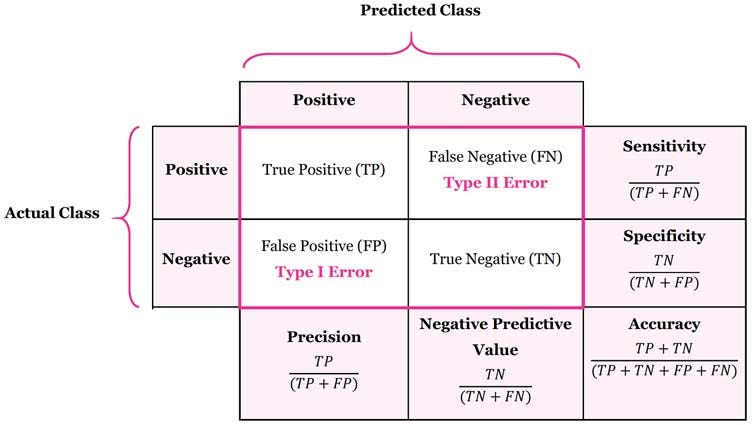
\includegraphics[width=0.95\textwidth, center]{images/contoh-confusion-matrix.jpg}
    \caption{Confusion Matrix}
    \label{fig:contoh-confusion-matrix} 
\end{afigure}
\textit{Confusion matrix} adalah alat evaluasi yang digunakan dalam klasifikasi statistik untuk menilai kinerja suatu model klasifikasi. Matriks ini memperlihatkan perbandingan antara hasil prediksi model dan hasil aktual dari data yang diuji. \textit{Confusion matrix} berfungsi untuk memberikan gambaran detail tentang bagaimana model melakukan klasifikasi, dengan mencakup empat komponen utama: True Positive (TP), True Negative (TN), False Positive (FP), dan False Negative (FN).

\begin{itemize}
    \item \textbf{True Positive (TP)}: Jumlah kasus di mana model memprediksi kelas positif dengan benar.
    \item \textbf{True Negative (TN)}: Jumlah kasus di mana model memprediksi kelas negatif dengan benar.
    \item \textbf{False Positive (FP)}: Jumlah kasus di mana model salah memprediksi kelas positif (Type I error).
    \item \textbf{False Negative (FN)}: Jumlah kasus di mana model salah memprediksi kelas negatif (Type II error).
\end{itemize}

\section{Jupyter Notebook}
Jupyter Notebook adalah aplikasi web open-source yang memungkinkan pengguna untuk membuat dan berbagi dokumen yang mengandung kode langsung, visualisasi, dan teks penjelasan. Jupyter Notebook sangat populer di kalangan ilmuwan data, peneliti, dan pengembang karena kemampuannya untuk mendukung analisis data interaktif dan komputasi ilmiah dalam berbagai bahasa pemrograman seperti Python, R, dan Julia. \cite{Jupyter2021}
Fitur Utama Jupyter Notebook:
\begin{enumerate}
    \item \textbf{Interaktif dan Real-Time}: Pengguna dapat menulis dan mengeksekusi kode langsung di dalam notebook, melihat hasilnya secara langsung. Hal ini memungkinkan eksperimen yang cepat dan interaktif.
    \item \textbf{Rich Media Integration}: Selain kode dan teks, Jupyter Notebook dapat menyertakan visualisasi data, gambar, video, dan bahkan widget interaktif, yang membantu dalam presentasi data yang lebih komprehensif dan mudah dipahami.
    \item \textbf{Reproducible Research}: Notebook dapat dibagikan dengan orang lain dan dieksekusi ulang untuk mendapatkan hasil yang sama, mendukung praktik penelitian yang dapat direproduksi.
    \item \textbf{Markdown Support}: Pengguna dapat menggunakan Markdown untuk menambahkan teks format, header, daftar, link, dan banyak lagi, membuat dokumen lebih rapi dan mudah dibaca.
    \item \textbf{Versi dan Kolaborasi}: Notebook disimpan dalam format file .ipynb yang dapat dengan mudah dipantau versi dan kolaborasi menggunakan sistem kontrol versi seperti Git.
    \item \textbf{Ekosistem Luas}: Jupyter mendukung berbagai jenis kernel untuk bahasa pemrograman yang berbeda, memperluas kemampuannya di luar Python saja.
\end{enumerate}

Contoh Penggunaan Jupyter Notebook: 
\begin{enumerate}
    \item \textbf{Data Analysis}: Analisis dataset besar menggunakan pustaka seperti Pandas, NumPy, dan SciPy.
    \item \textbf{Machine Learning}: Pembangunan dan pelatihan model machine learning menggunakan pustaka seperti scikit-learn, TensorFlow, dan PyTorch.
    \item \textbf{Visualization}: Membuat visualisasi data yang kompleks menggunakan Matplotlib, Seaborn, dan Plotly.
    \item \textbf{Education}: Digunakan sebagai alat pembelajaran interaktif untuk mengajarkan pemrograman dan konsep ilmu data.
\end{enumerate}

\section{Git}
Git adalah sistem kontrol versi terdistribusi yang dirancang untuk melacak perubahan pada file dan mengoordinasikan pekerjaan di antara beberapa orang. Git awalnya dikembangkan oleh Linus Torvalds pada tahun 2005 untuk mendukung pengembangan kernel Linux. Sistem ini sangat populer di kalangan pengembang perangkat lunak karena kemampuannya untuk menangani proyek besar dengan kecepatan dan efisiensi yang tinggi \cite{Git2024}.
Fitur Utama Git:
\begin{enumerate}
    \item \textbf{Distribusi}: Setiap klon dari repositori Git adalah repositori lengkap dengan riwayat lengkap dan kemampuan pelacakan versi penuh. Hal ini berarti setiap pengembang dapat bekerja secara offline dan melakukan sinkronisasi perubahan saat kembali online.
    \item \textbf{Branching dan Merging}: Git memungkinkan pembuatan cabang (branch) yang mudah dan efisien. Branching memungkinkan pengembang untuk bekerja pada fitur baru atau perbaikan bug secara terpisah dari cabang utama (main branch). Setelah selesai, cabang dapat digabungkan (merge) kembali ke cabang utama.
    \item \textbf{Kecepatan dan Kinerja}: Git dirancang untuk efisiensi dalam hal kecepatan dan performa. Operasi lokal seperti commit, diff, dan log sangat cepat karena tidak memerlukan komunikasi dengan server.
    \item \textbf{Keamanan}: Git menggunakan hashing SHA-1 untuk memastikan integritas konten dan riwayat perubahan, membuatnya sangat sulit untuk memanipulasi data tanpa terdeteksi.
    \item \textbf{Kolaborasi}: Git mendukung berbagai alur kerja kolaboratif, termasuk pengembangan terpusat, alur kerja GitHub, dan pengembangan berbasis cabang.
\end{enumerate}

\section{\textit{Image Normalization}}
\textit{Image normalization} adalah teknik yang digunakan dalam pemrosesan gambar dan pembelajaran mesin untuk menstandardisasi skala nilai piksel dalam gambar. Normalisasi gambar bertujuan untuk meningkatkan konvergensi dan performa model dengan memastikan bahwa data input berada dalam rentang yang seragam dan memiliki distribusi yang lebih stabil. Ini sangat penting dalam jaringan saraf konvolusional (CNN) dan metode pembelajaran mesin lainnya, di mana skala nilai yang tidak konsisten dapat mempengaruhi pembelajaran model \cite{Goodfellow-et-al-2016}.

Keuntungan \textit{Image Normalization}:
\begin{enumerate}
    \item \textbf{Konsistensi}: Membuat data lebih konsisten dan seragam, yang membantu model belajar dengan lebih efisien.
    \item \textbf{Konvergensi Lebih Cepat}: Membantu model neural network untuk berkonvergensi lebih cepat selama pelatihan.
    \item \textbf{Mengurangi Variabilitas}: Mengurangi efek variabilitas pencahayaan dan kontras dalam gambar.
\end{enumerate}

\section{\textit{Web Scraping}}
\textit{Web scraping} adalah teknik untuk mengekstrak data dari situs web secara otomatis menggunakan program atau bot. Proses ini melibatkan pengiriman permintaan ke server web, mengambil halaman web, dan kemudian menganalisis konten halaman tersebut untuk mengekstrak informasi yang diinginkan.\textit{ Web scraping} sering digunakan untuk mengumpulkan data dari internet dalam jumlah besar, yang kemudian dapat dianalisis atau digunakan untuk berbagai aplikasi \cite{Mitchell2018}. Google Image Scraper adalah contoh khusus dari web scraping yang digunakan untuk mengekstrak gambar dari hasil pencarian Google Images. \textit{Scraper} ini mengirimkan permintaan pencarian ke Google Images dan kemudian mengunduh gambar yang muncul dalam hasil pencarian.

\section{\textit{Good fit, Overfit, Underfit}}
\subsection{\textit{Good fit}}
Good fit terjadi ketika model statistik atau machine learning berhasil menangkap pola yang ada dalam data pelatihan dan mampu membuat prediksi yang akurat pada data baru (tidak terlihat). Model yang memiliki good fit menunjukkan keseimbangan yang baik antara bias dan variansi, artinya model tersebut cukup kompleks untuk menangkap pola data tetapi tidak terlalu kompleks sehingga mempelajari noise dalam data \cite{Goodfellow-et-al-2016}.
\subsection{\textit{Overfit}}
\textit{Overfitting} terjadi ketika model terlalu kompleks dan mulai belajar \textit{noise} atau variasi acak dalam data pelatihan sebagai informasi yang sebenarnya. Hal ini menyebabkan model memiliki performa yang sangat baik pada data pelatihan tetapi buruk pada data baru atau tidak terlihat. Model \textit{overfit} memiliki variansi yang tinggi dan bias yang rendah. \textit{Overfitting} dapat diidentifikasi melalui kinerja yang jauh lebih baik pada data pelatihan dibandingkan data validasi atau pengujian \cite{Goodfellow-et-al-2016}.

Menurut \cite{Desai2019}, model dikatakan mengalami \textit{overfit} jika dilatih secara berlebihan pada data sehingga model tersebut bahkan mempelajari \textit{noise} dari data tersebut. Model \textit{overfit} mempelajari setiap contoh dengan sangat sempurna sehingga salah mengklasifikasikan contoh yang tidak terlihat atau baru. Untuk model yang mengalami \textit{overfit}, memiliki skor set pelatihan yang sempurna atau mendekati sempurna, sementara skor pengujian atau validasi buruk.

\subsection{Underfit}
\textit{Underfitting} terjadi ketika model terlalu sederhana dan gagal menangkap pola dasar dalam data pelatihan. Ini berarti model tidak memiliki cukup kapasitas untuk memahami hubungan yang mendasari data, yang menyebabkan performa buruk baik pada data pelatihan maupun data baru. Model \textit{underfit} memiliki bias yang tinggi dan variansi yang rendah. \cite{Goodfellow-et-al-2016}

Menurut \cite{Desai2019}, Model dikatakan mengalami underfit jika tidak mampu mempelajari pola dalam data dengan baik. Model underfit tidak sepenuhnya mempelajari setiap contoh dalam dataset. Dalam kasus seperti ini, dapat dilihat skor yang rendah pada set pelatihan maupun set pengujian atau validasi.

\section{Mesin DGX}
Mesin DGX adalah platform komputasi yang dirancang oleh NVIDIA untuk mendukung aplikasi kecerdasan buatan (AI) dan pembelajaran mendalam (\textit{deep learning}). Mesin DGX menyediakan infrastruktur yang kuat dan efisien untuk melakukan pelatihan model AI yang kompleks, memungkinkan peneliti dan praktisi untuk mempercepat pengembangan dan implementasi solusi AI.

DGX dilengkapi dengan GPU NVIDIA yang kuat, memori besar, dan perangkat lunak yang dioptimalkan untuk AI, seperti NVIDIA CUDA dan cuDNN. Ini menjadikan DGX sebagai pilihan utama untuk berbagai aplikasi AI, mulai dari pengenalan gambar hingga pemrosesan bahasa alami \cite{NVIDIA2021}.

Universitas Gunadarma menghadirkan mesin super komputer Nvidia DGX-1 dan DGX A100 di Indonesia. Mesin super komputer Nvidia DGX-1 dan DGX A100 merupakan mesin dengan kemampuan tinggi dalam melakukan proses dengan jumlah data besar, mendukung dalam perkembangan \textit{Big Data}, \textit{Data Analytic}, dan \textit{Artificial Intelligence}. 

Mesin Nvidia DGX-1 merupakan mesin dengan 8 (delapan) GPU dan masing-masing memiliki 16 GB memory. Mesin DGX A100 merupakan mesin dengan 8 (delapan) GPU dan total 320 GB memory, serta memiliki 6 (enam) Nvidia NVSwitches.

Mesin Nvidia DGX-1 memiliki kemampuan 56 kali lebih baik daripada CPU, dan 75 kali kecepatan dalam melakukan pelatihan. Mesin Nvidia DGX A100 memiliki kemampuan 172 kali lebih baik daripada CPU server, dan juga kemampuan training, inference, serta data analytic \cite{HPCGunadarma}.







    \chapter{METODE PENELITIAN}

Metode pada penelitian ini terdiri dari beberapa tahapan proses seperti yang terlihat pada Gambar 3.1.
%\begin{afigure}
%    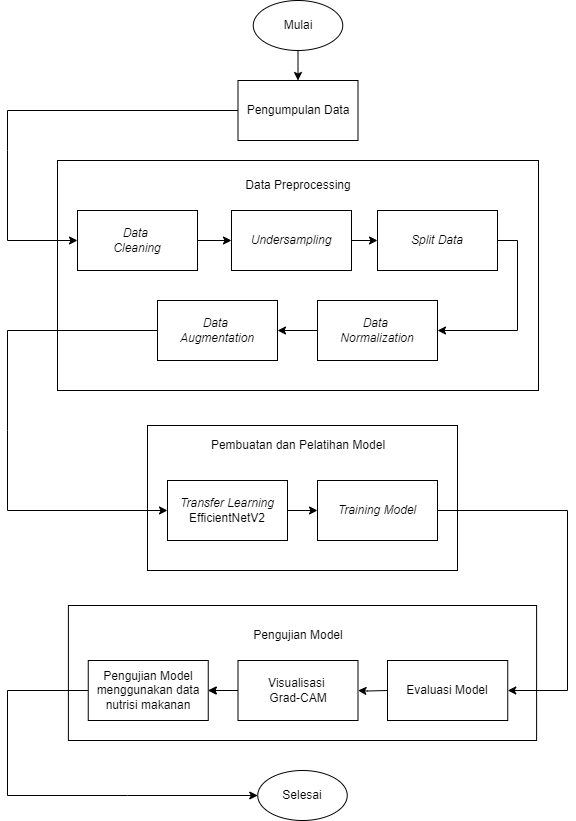
\includegraphics[height=0.74\textheight, width=0.9\textwidth, center]{images/flowchart.png}
%    \caption{Flowchart Tahapan Metode Penelitian}
%    \label{fig:flowchart-metode}
%\end{afigure}






    \chapter{HASIL DAN PEMBAHASAN}

Setelah dilakukan penjelasan terhadap langkah-langkah mulai dari pengumpulan data, \textit{data preprocessing}, Pembuatan dan Pelatihan Model, dan Pengujian Model. Selanjutnya, menampilkan hasil dari tahapan-tahapan tersebut. Kinerja model klasifikasi dalam melakukan pengklasifikasian juga akan diperlihatkan untuk mengukur seberapa baik model tersebut dalam mengklasifikasikan citra makanan. \textit{Confussion matrix} dan \textit{classification report} akan digunakan sebagai alat ukur untuk evaluasi pada klasifikasi citra makanan tersebut. Semakin tinggi akurasi klasifikasi berarti performa klasifikasi juga semakin baik.

\section{Hasil Pengumpulan Data}
Hasil pengumpulan data citra makanan yang diperoleh menggunakan teknik \textit{Scraping} berjumlah sebanyak 5000 citra makanan yang terbagi dalam 10 kelas (ayam bakar, bakso, gado gado, gudeg, nasi goreng, pempek, rawon, rendang, sate, dan soto), dimana setiap kelas memiliki total 500 citra makanan.

\begin{afigure}
    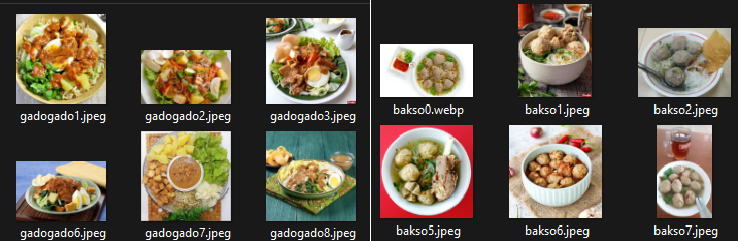
\includegraphics[width=0.95\textwidth, center]{images/citra-makanan.png}
    \caption{Hasil pengumpulan data citra makanan}
    \label{fig:citra-makanan}
\end{afigure}

Gambar 4.1 merupakan contoh data citra makanan yang berhasil dikumpulkan menggunakan teknik \textit{scraping} dalam penelitian ini. Gambar 4.1 menunjukan perbedaan signifikan dari gado-gado dan bakso. Perbedaan signifikan tersebut meliputi bentuk dan warna.

\section{Hasil \textit{Data Preprocessing}}
Hasil dari \textit{data preprocessing} terbagi menjadi menjadi 4 bagian, yaitu:
\begin{enumerate}
    \item Hasil \textit{Data Cleaning}.
    \item Hasil \textit{Undersampling}.
    \item Hasil \textit{Split Data}.
    \item Hasil \textit{Data Normalization} dan \textit{Data Augmentation}.
\end{enumerate}

\subsection{Hasil \textit{Data Cleaning}}
Setelah data berhasil dikumpulkan menggunakan teknik \textit{scraping}, kemudian dilakukan proses \textit{Data Cleaning}. Tahap ini akan memperlihatkan hasil dari \textit{data cleaning}. Berikut hasil dari \textit{data cleaning} pada Tabel 4.1

\begin{atable}
    \centering
    \caption{Hasil Cleaning Data}
    \label{table:hasil-cleaning}
    \csvreader[
        head to column names,
        separator=semicolon,
        tabular={|c|c|},
        table head=\hline
            \rowcolor{gray!50!black}
            \color{white} Makanan & 
            \color{white} Jumlah Data \\ \hline,
        late after line=\\ \hline,
        late after last line=\\ \hline
        ]
        {tables/cleaning.csv}
        {makanan=\makanan, jumlah=\jumlah}
        {\makanan & \jumlah}
\end{atable}

Hal ini dilakukan karena data citra yang didapatkan dari \textit{scraping} banyak yang \textit{duplicate} dan banyak citra yang tidak sesuai dengan makanan yang dimaksud. \textit{Data Cleaning} dilakukan agar dapat memastikan konsistensi data dan model dapat mengenali data yang benar.

\subsection{Hasil \textit{Undersampling}}
Setelah melakukan \textit{data cleaning}, langkah berikutnya adalah \textit{Undersampling} pada data. \textit{Undersampling} dilakukan untuk menangani ketidakseimbangan data yang ada dalam dataset. Ketidakseimbangan data terjadi ketika jumlah citra dalam satu kelas makanan jauh lebih banyak dibandingkan dengan kelas lainnya. Hasil \textit{Undersampling} dapat dilihat pada Tabel 4.2.

\begin{atable}
    \centering
    \caption{Hasil Undersampling}
    \label{table:hasil-undersampling}
    \csvreader[
        head to column names,
        separator=semicolon,
        tabular={|c|c|c|},
        table head=\hline
            \rowcolor{gray!50!black}
            \color{white} Makanan & 
            \color{white} Jumlah Sebelum Undersampling &
            \color{white} Jumlah Sesudah Undersampling \\ \hline,
        late after line=\\ \hline,
        late after last line=\\ \hline
        ]
        {tables/undersampling.csv}
        {makanan=\makanan, sebelum=\sebelum, sesudah=\sesudah}
        {\makanan & \sebelum & \sesudah}
\end{atable}

Setelah dilakukan \textit{Undersampling}, semua data pada tiap kelas menjadi 200 citra. \textit{Undersampling} dilakukan untuk mengurangi adanya bias. Bias biasa terjadi ketika terjadi ketidakseimbangan data.

\subsection{Hasil \textit{Split Data}}
Setelah dilakukan proses \textit{Undersampling}, data kemudian dibagi menjadi menjadi data latih dan data uji. Berikut hasil \textit{Split Data} pada Gambar 4.2.

\begin{afigure}
    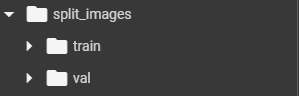
\includegraphics[width=0.5\textwidth, center]{images/hasil-split.png}
    \caption{Hasil Split Data}
    \label{fig:hasil-split}
\end{afigure}
Setelah dilakukan \textit{Split Data}, dataset sekarang mempunyai 2 bagian, yaitu data latih dan data uji. Dengan rasio 80\% untuk data latih, dan 20\% untuk data uji, data latih mempunyai 160 citra tiap kelasnya, sedangkan data uji mempunyai 40 citra tiap kelasnya.

\subsection{Hasil \textit{Data Normalization} dan \textit{Data Augmentation}}
Setelah dilakukan \textit{Split Data} menjadi data uji dan data latih, kemudian dilakukan proses \textit{Data Normalization} dan \textit{Data Augmentation}. Berikut contoh dataset sebelum dilakukan proses \textit{Data Normalization} dan \textit{Data Augmentation} pada Gambar 4.3.

\begin{afigure}
    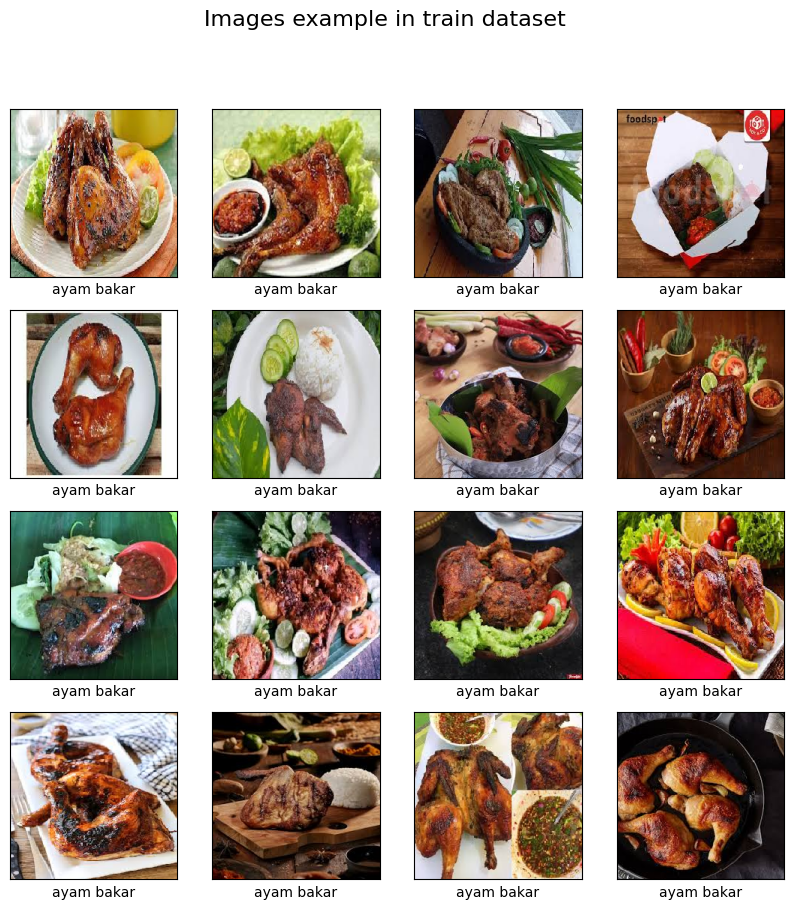
\includegraphics[height=0.6\textheight, width=0.9\textwidth, center]{images/raw-dataset.png}
    \caption{Data Sebelum Proses \textit{Data Normalization} dan \textit{Data Augmentation}}
    \label{fig:sebelum-augmentasi}
\end{afigure}

\begin{afigure}
    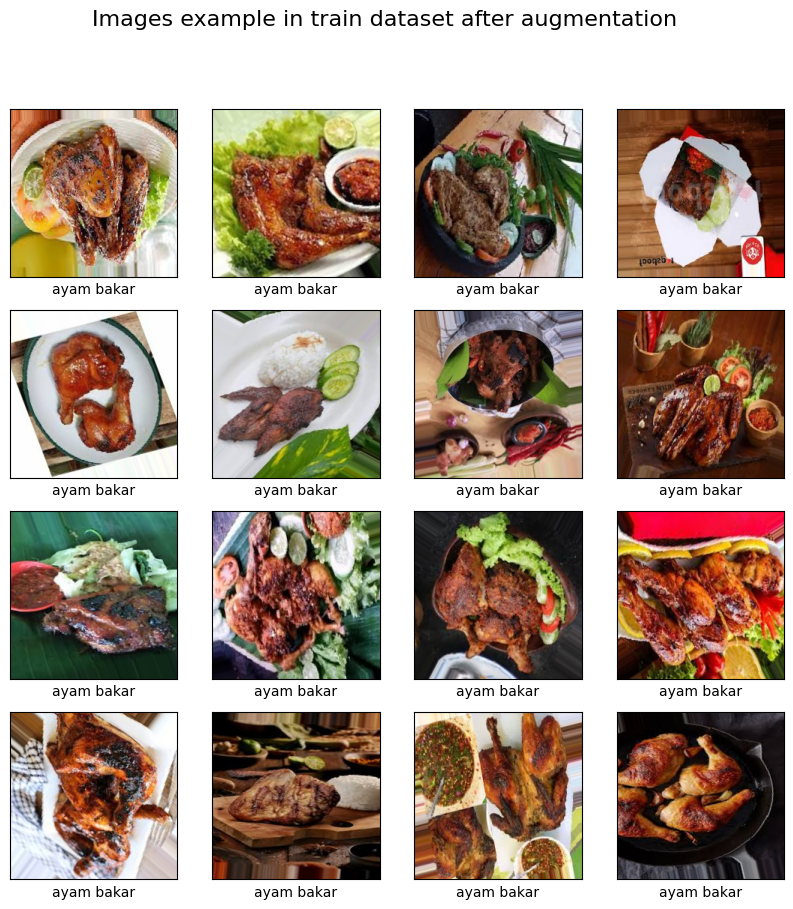
\includegraphics[height=0.6\textheight, width=0.9\textwidth, center]{images/augmented.png}
    \caption{Data Sesudah Proses \textit{Data Normalization} dan \textit{Data Augmentation}}
    \label{fig:sesudah-augmentasi}
\end{afigure}

Pada Gambar 4.4, terlihat citra yang telah dilakukan proses \textit{Data Normalization} dan \textit{Data Augmentation} terlihat berbeda dengan sebelumnya. Setelah dilakukan proses tersebut, terlihat beberapa citra terbalik secara vertikal ataupun horizontal, beberapa citra mengalami rotasi, dan beberapa citra diperbesar.

\section{Hasil Pembuatan dan Pelatihan Model}
Setelah dilakukan proses \textit{Data Preprocessing}, kemudian dilakukan proses Pembuatan dan Pelatihan Model. Hasil Pembuatan dan Pelatihan Model dibagi menjadi 2 bagian, yaitu:
\begin{enumerate}
    \item Hasil \textit{Transfer Learning} EfficientNetV2
    \item Hasil \textit{Training Model}
\end{enumerate}

\subsection{Hasil \textit{Transfer Learning} EfficientNetV2}
\begin{afigure}
    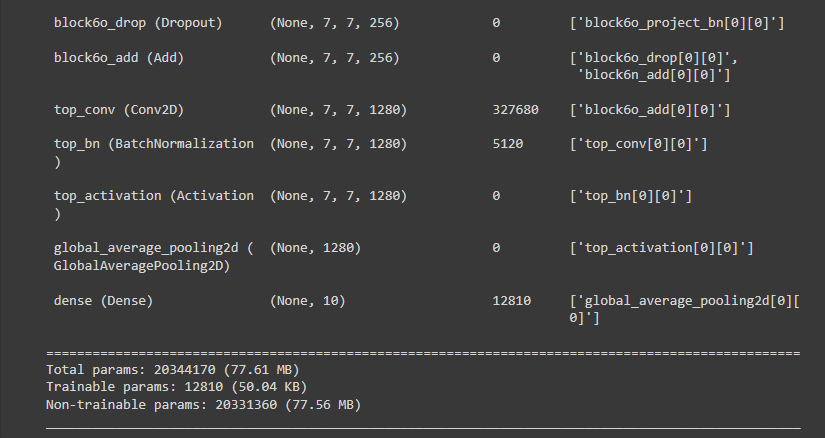
\includegraphics[width=0.9\textwidth, center]{images/model-summary.png}
    \caption{Ringkasan Model Hasil Transfer Learning EfficientNetV2}
    \label{fig:model-summary}
\end{afigure}

Gambar 4.5 merupakan ringkasan dari model yang telah dibuat. Pada penelitian ini, model yang telah dibuat menggunakan \textit{layer} dari EfficientNetV2, lalu ditambahkan lapisan tambahan yaitu lapisan GlobalAveragePooling2D dan lapisan Dense dengan aktivasi softmax. Berikut adalah penjelasan dari parameter yang terdapat dalam Gambar 4.5:

\begin{itemize}
    \item \textbf{Total params: 20,344,170 (77.61 MB)}: Ini adalah jumlah total parameter dalam model yang telah dibuat. Parameter ini mencakup semua bobot (\textit{weights}) dan bias (\textit{biases}) yang ada di dalam model, baik yang dapat dilatih maupun yang tidak dapat dilatih.
    \item \textbf{Trainable params: 12,810 (50.04 KB)}: Ini adalah jumlah parameter yang dapat dilatih dalam model yang telah dibuat. Dalam kasus ini, hanya ada 12,810 parameter yang dapat dilatih. Parameter ini berasal dari lapisan tambahan yang ditambahkan setelah model pra-latih EfficientNetV2S, yaitu lapisan GlobalAveragePooling2D dan lapisan Dense dengan aktivasi softmax.
    \item \textbf{Non-trainable params: 20,331,360 (77.56 MB)}: Ini adalah jumlah parameter yang tidak dapat dilatih. Parameter ini merupakan parameter dari model pra-latih EfficientNetV2S yang digunakan. Karena diatur pre\_trained\_model.trainable = False, parameter dalam EfficientNetV2S tidak akan diperbarui selama pelatihan.
\end{itemize}

\subsection{Hasil \textit{Training Model}}
Setelah dilakukan pembuatan model dengan menggunakan metode \textit{transfer learning}, kemudian dilakukan proses \textit{training model} atau pelatihan model. Pada penelitian ini, model dilatih menggunakan \textit{learning rate} sebesar 0.001, callback ModelCheckPoint untuk menyimpan model terbaik berdasarkan val\_loss terkecil, dan menggunakan epoch sebanyak 50 epoch. 
Hasil \textit{Training Model} dibagi menjadi 2 bagian, yaitu:
\begin{enumerate}
    \item Hasil \textit{Training Model} menggunakan Google Colab GPU T4
    \item Hasil \textit{Training Model} menggunakan mesin DGX A100 Universitas Gunadarma.
\end{enumerate}

\subsubsection{Hasil \textit{Training Model} menggunakan Google Colab GPU T4}
Berikut tabel hasil pelatihan model menggunakan Google Colab GPU T4 dengan konfigurasi tersebut:
\begin{longtable}{|c|c|c|c|c|}
    \caption{Hasil Training Model menggunakan Google Colab GPU T4} \label{table:hasil-training} \\ \hline
    \rowcolor{gray!50!black}
    \color{white} Epoch &
    \color{white} Loss & 
    \color{white} Accuracy &
    \color{white} Val Loss &
    \color{white} Val Accuracy \\ \hline
    \endfirsthead
    
    \hline
    \rowcolor{gray!50!black}
    \color{white} Epoch &
    \color{white} Loss & 
    \color{white} Accuracy &
    \color{white} Val Loss &
    \color{white} Val Accuracy \\ \hline
    \endhead
    
    \csvreader[
        head to column names,
        late after line=\\ \hline,
        late after last line=\\ \hline
        ]
        {tables/training-history.csv}
        {loss=\loss, accuracy=\accuracy, val_loss=\valloss, val_accuracy=\valaccuracy}
        {%
            \ifthenelse{\equal{\thecsvrow}{49}}{%
                \bfseries\thecsvrow & \bfseries\num{\loss} & \bfseries\num{\accuracy} & \bfseries\num{\valloss} & \bfseries\num{\valaccuracy}%
            }{%
                \thecsvrow & \num{\loss} & \num{\accuracy} & \num{\valloss} & \num{\valaccuracy}%
            }%
        }
\end{longtable}

Tabel 4.3 merupakan hasil pelatihan model menggunakan Google Colab GPU T4 sebanyak 50 epoch. Model terbaik yang diambil merupakan model dengan \textit{Val Loss} terkecil, berdasarkan hasil pelatihan model pada Tabel 4.3, model terbaik merupakan model pada Epoch ke-49, dengan \textit{Val Loss} sebesar 0.3944 dan \textit{Val Accuracy} sebesar 0.8750 atau 87.50\%. Dengan menggunakan Google Colab GPU T4, pelatihan memakan waktu selama 22 menit.

\subsubsection{Hasil \textit{Training Model} menggunakan mesin DGX A100 Universitas Gunadarma}
Berikut tabel hasil pelatihan model menggunakan mesin DGX A100 Universitas Gunadarma dengan konfigurasi tersebut:
\begin{longtable}{|c|c|c|c|c|}
    \caption{Hasil Training Model menggunakan mesin DGX A100 Universitas Gunadarma} \label{table:hasil-training-dgx} \\ \hline
    \rowcolor{gray!50!black}
    \color{white} Epoch &
    \color{white} Loss & 
    \color{white} Accuracy &
    \color{white} Val Loss &
    \color{white} Val Accuracy \\ \hline
    \endfirsthead
    
    \hline
    \rowcolor{gray!50!black}
    \color{white} Epoch &
    \color{white} Loss & 
    \color{white} Accuracy &
    \color{white} Val Loss &
    \color{white} Val Accuracy \\ \hline
    \endhead
    
    \csvreader[
        head to column names,
        late after line=\\ \hline,
        late after last line=\\ \hline
        ]
        {tables/training-history-dgx.csv}
        {loss=\loss, accuracy=\accuracy, val_loss=\valloss, val_accuracy=\valaccuracy}
        {%
            \ifthenelse{\equal{\thecsvrow}{50}}{%
                \bfseries\thecsvrow & \bfseries\num{\loss} & \bfseries\num{\accuracy} & \bfseries\num{\valloss} & \bfseries\num{\valaccuracy}%
            }{%
                \thecsvrow & \num{\loss} & \num{\accuracy} & \num{\valloss} & \num{\valaccuracy}%
            }%
        }
\end{longtable}

Tabel 4.4 merupakan hasil pelatihan model menggunakan mesin DGX A100 Universitas Gunadarma sebanyak 50 epoch. Model terbaik yang diambil merupakan model dengan \textit{Val Loss} terkecil, berdasarkan hasil pelatihan model pada Tabel 4.4, model terbaik merupakan model pada Epoch ke-50, dengan \textit{Val Loss} sebesar 0.3925 dan \textit{Val Accuracy} sebesar 0.8725 atau 87.25\%. Dengan menggunakan mesin DGX A100 Universitas Gunadarma, pelatihan memakan waktu selama 11 menit saja.

\section{Hasil Pengujian Model}
Setelah melalui tahap \textit{Training Model}, kemudian dilakukan tahap terakhir yaitu Pengujian Model. Hasil Pengujian Model dibagi menjadi 2 bagian, yaitu:
\begin{enumerate}
    \item Hasil Pengujian Model Google Colab GPU T4
    \item Hasil Pengujian Model mesin DGX A100 Universitas Gunadarma
\end{enumerate}

\subsection{Hasil Pengujian Model Google Colab GPU T4}
Hasil Pengujian Model Google Colab GPU T4 dibagi menjadi 3 bagian, yaitu:
\begin{enumerate}
    \item Hasil Evaluasi Model
    \item Hasil Visualisasi Grad-CAM
    \item Hasil Pengujian Model menggunakan data nutrisi makanan
\end{enumerate}

\subsubsection{Hasil Evaluasi Model}
Tahap pertama pada Evaluasi Model yaitu untuk mengetahui model tersebut termasuk \textit{overfit, good fit} atau \textit{underfit}. Untuk mengetahui hal tersebut, dapat dilakukan dengan membuat visualisasi dari hasil pelatihan model dengan diagram garis. Berikut hasil visualisasi pelatihan model dengan diagram garis:

\begin{afigure}
    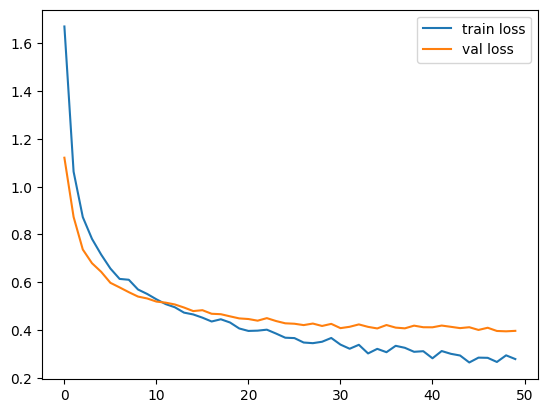
\includegraphics[height=0.4\textheight, width=0.9\textwidth, center]{images/train-loss.png}
    \label{fig:train-loss}
\end{afigure}
\pagebreak
\begin{afigure}
    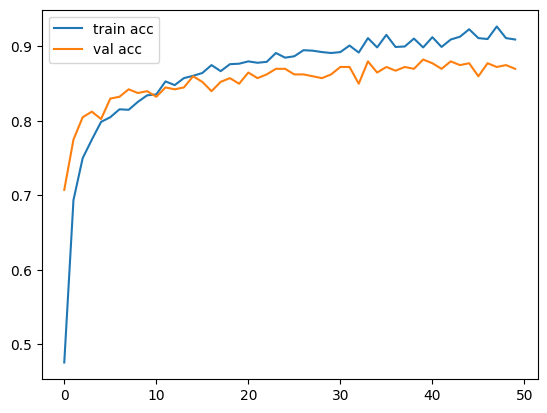
\includegraphics[height=0.4\textheight, width=0.9\textwidth, center]{images/train-acc.png}
    \caption{Visualisasi Pelatihan Model Google Colab GPU T4}
    \label{fig:train-acc}
\end{afigure}

Pada Gambar 4.6, terlihat \textit{train loss} dan \textit{val loss} mendekati satu sama lain dan terus menurun hingga datar dari beberapa titik hingga akhir. Kemudian, \textit{train acc} dan \textit{val acc} juga mendekati satu sama lain. Hal ini dapat diartikan bahwa model tersebut termasuk \textit{good fit} dan layak dipakai.

Setelah mengetahui bahwa model layak dipakai, kemudian dilakukan \textit{
Classification Report} untuk mengetahui performa model berdasarkan metriks \textit{precision}, \textit{recall}, dan \textit{F1-Score}. Berikut hasil dari \textit{Classification Report} menggunakan \textit{library} dari sklearn:

\pagebreak

\begin{afigure}
    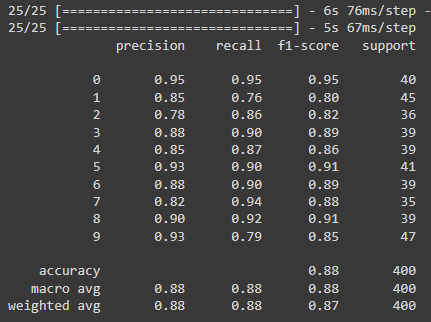
\includegraphics[width=0.9\textwidth, center]{images/classification-report.png}
    \caption{Hasil Classification Report Model Google Colab GPU T4}
    \label{fig:classification-report}
\end{afigure}


\begin{itemize}
    \item Accuracy: 0.88, menunjukkan bahwa model ini memiliki tingkat akurasi 88\% di seluruh kelas.
    \item Macro Avg: Rata-rata precision, recall, dan f1-score untuk setiap kelas, tanpa mempertimbangkan jumlah instance di setiap kelas.
    \item Weighted Avg: Rata-rata precision, recall, dan f1-score untuk setiap kelas, dengan mempertimbangkan jumlah instance di setiap kelas.
\end{itemize}

Gambar 4.7 menunjukan bahwa model memiliki performa yang baik di sebagian besar kelas, meskipun ada beberapa kelas yang memiliki nilai \textit{recall} atau \textit{precision} yang lebih rendah. Ada beberapa citra yang salah diklasifikasikan ke kelas lain, contohnya pada kelas 1 (bakso), dan kelas 9 (soto).

Setelah dilakukan \textit{Classification Report}, untuk mempermudah evaluasi model dapat menggunakan \textit{confusion matrix}. Berikut visualisasi menggunakan \textit{confusion matrix}:

\begin{afigure}
    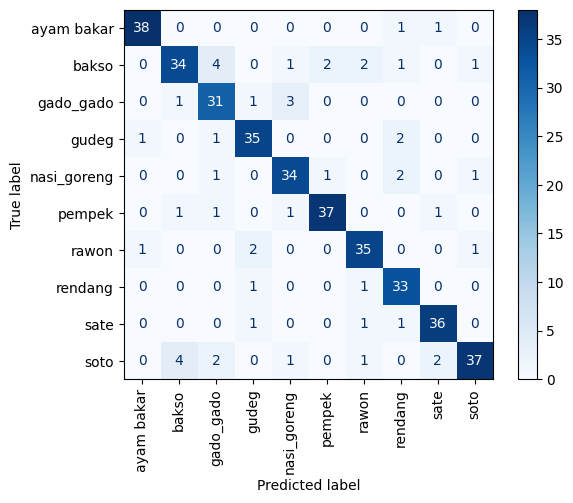
\includegraphics[width=0.9\textwidth, center]{images/confussion-matrix.png}
    \caption{Visualisasi Confusion Matrix Model Google Colab GPU T4}
    \label{fig:confussion-matrix}
\end{afigure}

Confusion matrix ini menunjukkan hasil dari model klasifikasi yang telah diuji dengan beberapa kategori makanan Indonesia. Berikut adalah interpretasi dari setiap elemen dalam \textit{confusion matrix} ini:
\begin{itemize}
    \item \textit{True label} (label sebenarnya) berada pada sumbu Y (vertikal).
    \item \textit{Predicted label} (label prediksi) berada pada sumbu X (horizontal).
\end{itemize}

Setiap sel dalam matriks menunjukkan jumlah instance yang diprediksi dalam kategori tertentu. Misalnya, sel pada baris "ayam bakar" dan kolom "ayam bakar" menunjukkan jumlah instance "ayam bakar" yang diprediksi benar oleh model. Berikut adalah beberapa poin penting yang dapat diperhatikan dari \textit{confusion matrix} pada Gambar 4.8:
\begin{itemize}
    \item \textbf{Ayam Bakar}: Dari 40 instance "ayam bakar", 38 diprediksi benar sebagai "ayam bakar", 1 diprediksi sebagai "gudeg", dan 1 diprediksi sebagai "rawon".
    \item \textbf{Bakso}: Dari 40 instance "bakso", 34 diprediksi benar sebagai "bakso", namun ada beberapa yang salah prediksi ke "gado-gado", "pempek", dan "soto".
    \item \textbf{Gado-gado}: Dari 40 instance "gado-gado", 31 diprediksi benar, namun ada beberapa yang salah prediksi ke "bakso", "gudeg", "nasi goreng", "pempek", dan "soto".
    \item \textbf{Gudeg}: Dari 40 instance "gudeg", 35 diprediksi benar, namun ada beberapa yang salah prediksi ke "gado-gado", "rawon", "rendang", dan "sate".
    \item \textbf{Nasi Goreng}: Dari 40 instance "nasi goreng", 34 diprediksi benar, namun ada beberapa yang salah prediksi ke "bakso", "gado-gado", dan "pempek", dan "soto".
    \item \textbf{Pempek}: Dari 40 instance "pempek", 37 diprediksi benar, namun ada beberapa yang salah prediksi ke "bakso" dan "nasi goreng".
    \item \textbf{Rawon}: Dari 40 instance "rawon", 35 diprediksi benar, namun ada beberapa yang salah prediksi ke "bakso", "rendang", "sate", dan "soto".
    \item \textbf{Rendang}: Dari 40 instance "rendang", 33 diprediksi benar, namun ada beberapa yang salah prediksi ke "ayam bakar", "bakso", , "gudeg", "nasi goreng", "rawon", dan "sate".
    \item \textbf{Sate}: Dari 40 instance "sate", 36 diprediksi benar, namun ada beberapa yang salah prediksi ke "ayam bakar", "pempek", dan "soto".
    \item \textbf{Soto}: Dari 40 instance "soto", 37 diprediksi benar, namun ada beberapa yang salah prediksi ke "bakso", "nasi goreng", dan "rawon".
\end{itemize}

Secara keseluruhan, model menunjukkan performa yang cukup baik dengan sebagian besar prediksi berada di diagonal utama, yang berarti banyak instance yang diklasifikasikan dengan benar. Namun, ada beberapa kesalahan prediksi yang perlu diperhatikan untuk meningkatkan akurasi model lebih lanjut.

\subsubsection{Hasil Visualisasi Grad-CAM}
Setelah melakukan proses Evaluasi Model, selanjutnya dilakukan proses Visualisasi Grad-CAM. Hal ini dilakukan untuk mengetahui bagaimana model melihat citra dan area mana yang dianggap penting oleh model dalam membuat prediksi. Berikut hasil visualisasi menggunakan Grad-CAM:

\begin{afigure}
    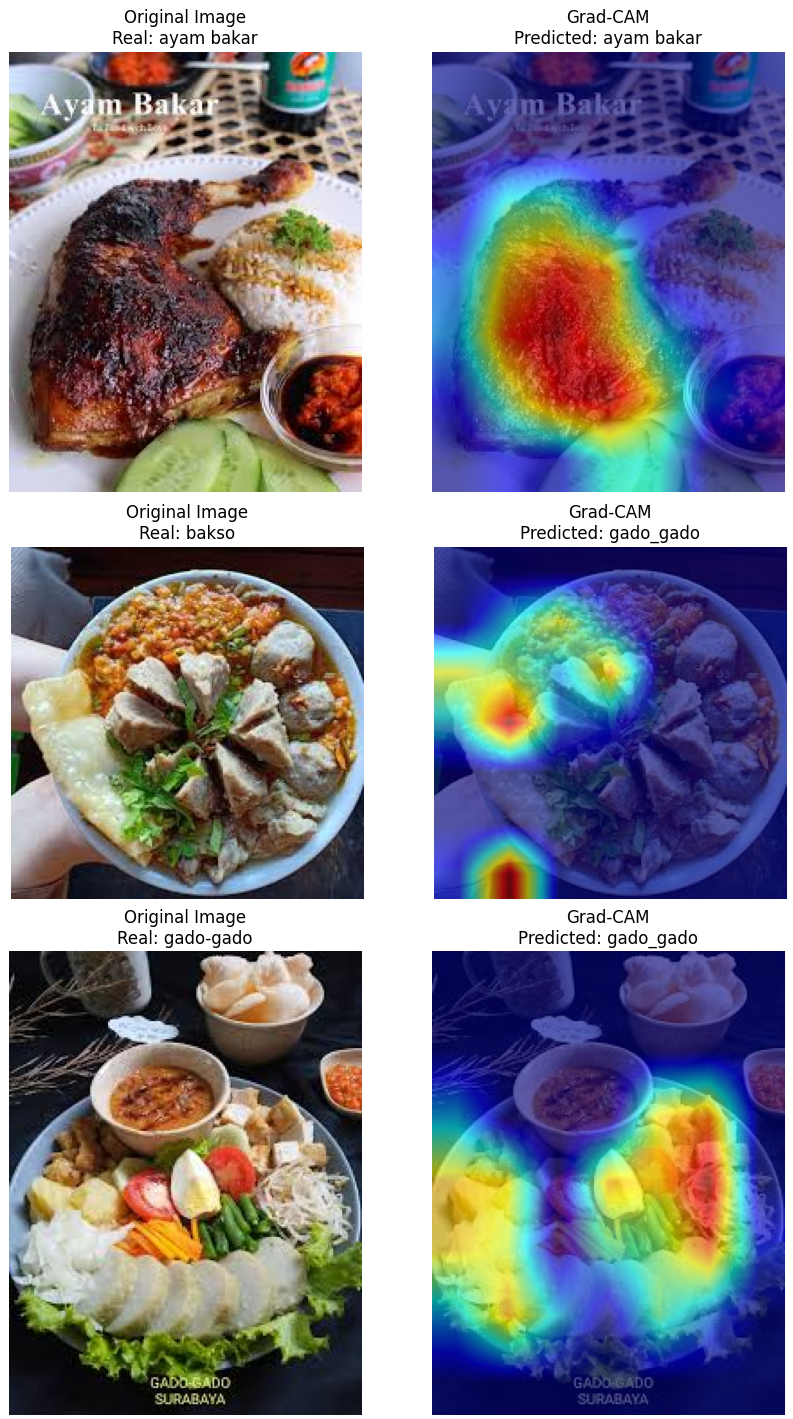
\includegraphics[height=0.75\textheight, width=0.9\textwidth, center]{images/grad-cam-1.png}
    \label{fig:grad-cam-1}
\end{afigure}
\clearpage
\begin{afigure}
    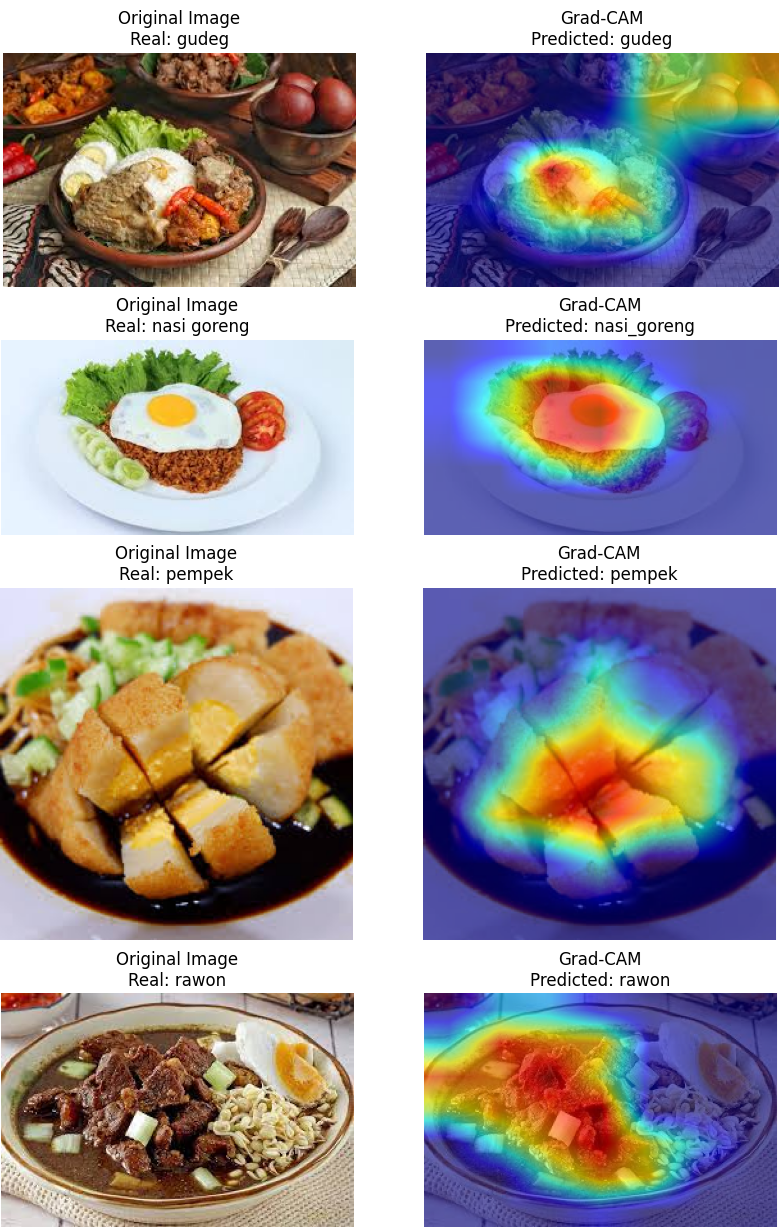
\includegraphics[width=0.9\textwidth, center]{images/grad-cam-2.png}
    \label{fig:grad-cam-2}
\end{afigure}
\clearpage
\begin{afigure}
    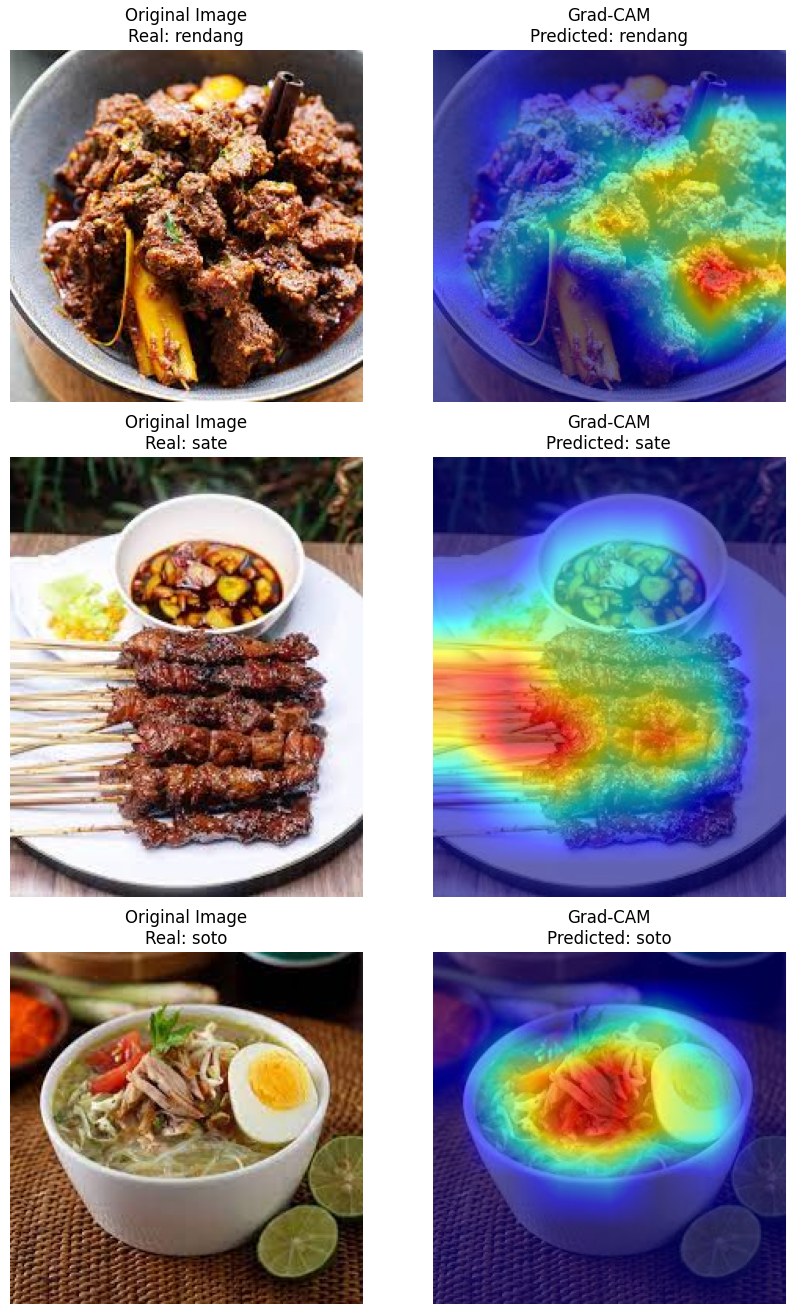
\includegraphics[width=0.9\textwidth, center]{images/grad-cam-3.png}
    \caption{Hasil Visualisasi Grad-CAM Model Google Colab GPU T4}
    \label{fig:grad-cam-3}
\end{afigure}

\clearpage

Pada Gambar 4.9, terlihat bahwa model mampu mengklasifikasikan 9 dari 10 citra dengan tepat. Namun, terdapat satu kelas yang memerlukan perhatian lebih lanjut, yaitu kelas bakso. Dalam visualisasi tersebut, kelas bakso diklasifikasikan sebagai gado-gado. Hal ini menunjukkan bahwa model mengalami kesulitan dalam membedakan antara kedua jenis makanan tersebut.

\subsubsection{Hasil Pengujian Model menggunakan data nutrisi makanan}
Setelah memastikan model memiliki performa yang bagus, selanjutnya dilakukan uji coba menggunakan data nutrisi makanan. Makanan yang berhasil diklasifikasikan kemudian akan ditampilkan informasi nutrisi pada makanan tersebut. Berikut hasil dari uji coba model menggunakan data nutrisi makanan: 
\begin{afigure}
    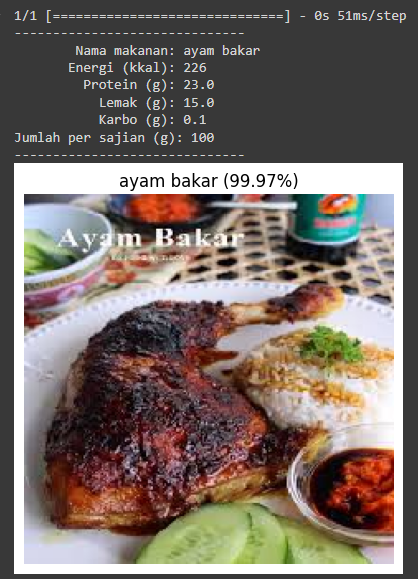
\includegraphics[height=0.55\textheight, width=0.9\textwidth, center]{images/predict-1.png}
    \label{fig:predict-1}
\end{afigure}
\pagebreak
\begin{afigure}
    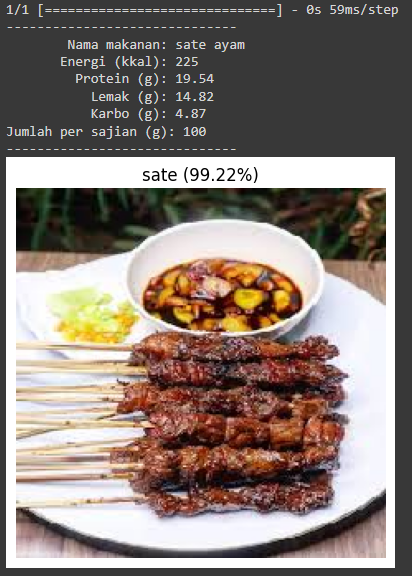
\includegraphics[height=0.55\textheight, width=0.9\textwidth, center]{images/predict-2.png}
    \caption{Hasil Pengujian Model Google Colab GPU T4 menggunakan data nutrisi makanan}
    \label{fig:predict-2}
\end{afigure}

Pada Gambar 4.10 terlihat bahwa model dapat digunakan dan informasi nutrisi dapat ditampilkan dengan baik. Citra juga berhasil diklasifikasikan dengan tepat, citra pertama berhasil diklasifikasikan sebagai ayam bakar dengan \textit{confidence} sebesar 99.97\%, kemudian citra kedua berhasil diklasifikasikan sebagai sate dengan \textit{confidence} sebesar 99.92\%.

\subsection{Hasil Pengujian Model mesin DGX A100 Universitas Gunadarma}
Hasil Pengujian Model mesin DGX A100 Universitas Gunadarma dibagi menjadi 3 bagian, yaitu:
\begin{enumerate}
    \item Hasil Evaluasi Model
    \item Hasil Visualisasi Grad-CAM
    \item Hasil Pengujian Model menggunakan data nutrisi makanan
\end{enumerate}

\subsubsection{Hasil Evaluasi Model}
Tahap pertama pada Evaluasi Model yaitu untuk mengetahui model tersebut termasuk \textit{overfit, good fit} atau \textit{underfit}. Untuk mengetahui hal tersebut, dapat dilakukan dengan membuat visualisasi dari hasil pelatihan model dengan diagram garis. Berikut hasil visualisasi pelatihan model dengan diagram garis:

\begin{afigure}
    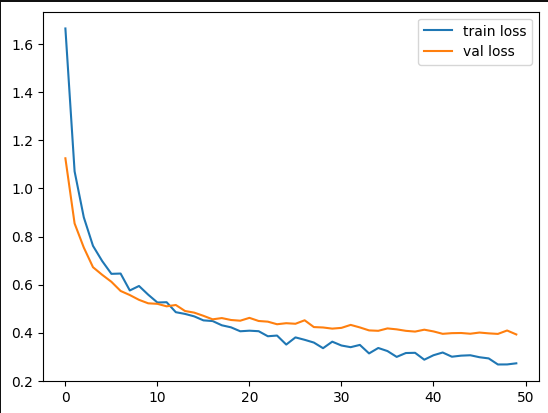
\includegraphics[height=0.4\textheight, width=0.9\textwidth, center]{images/train-loss-dgx.png}
    \label{fig:train-loss-dgx}
\end{afigure}
\pagebreak
\begin{afigure}
    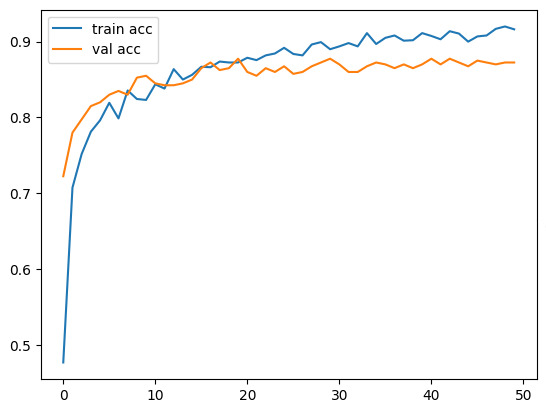
\includegraphics[height=0.4\textheight, width=0.9\textwidth, center]{images/train-acc-dgx.png}
    \caption{Visualisasi Pelatihan Model mesin DGX A100 Universitas Gunadarma}
    \label{fig:train-acc-dgx}
\end{afigure}

Pada Gambar 4.11, terlihat \textit{train loss} dan \textit{val loss} mendekati satu sama lain dan terus menurun hingga datar dari beberapa titik hingga akhir. Kemudian, \textit{train acc} dan \textit{val acc} juga mendekati satu sama lain. Hal ini dapat diartikan bahwa model tersebut termasuk \textit{good fit} dan layak dipakai.

Setelah mengetahui bahwa model layak dipakai, kemudian dilakukan \textit{
Classification Report} untuk mengetahui performa model berdasarkan metriks \textit{precision}, \textit{recall}, dan \textit{F1-Score}. Berikut hasil dari \textit{Classification Report} menggunakan \textit{library} dari sklearn:

\pagebreak

\begin{afigure}
    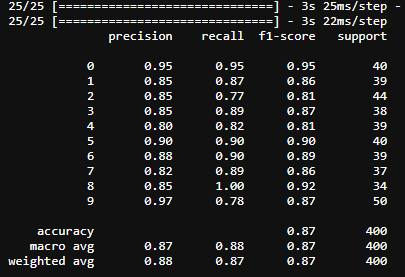
\includegraphics[width=0.9\textwidth, center]{images/classification-report-dgx.png}
    \caption{Hasil Classification Report Model mesin DGX A100 Universitas Gunadarma}
    \label{fig:classification-report-dgx}
\end{afigure}


\begin{itemize}
    \item Accuracy: 0.87, menunjukkan bahwa model ini memiliki tingkat akurasi 88\% di seluruh kelas.
    \item Macro Avg: Rata-rata precision, recall, dan f1-score untuk setiap kelas, tanpa mempertimbangkan jumlah instance di setiap kelas.
    \item Weighted Avg: Rata-rata precision, recall, dan f1-score untuk setiap kelas, dengan mempertimbangkan jumlah instance di setiap kelas.
\end{itemize}

Gambar 4.12 menunjukan bahwa model memiliki performa yang baik di sebagian besar kelas, meskipun ada beberapa kelas yang memiliki nilai \textit{recall} atau \textit{precision} yang lebih rendah. Ada beberapa citra yang salah diklasifikasikan ke kelas lain, contohnya pada kelas 2 (gado-gado) dan kelas 9 (soto).

Setelah dilakukan \textit{Classification Report}, untuk mempermudah evaluasi model dapat menggunakan \textit{confusion matrix}. Berikut visualisasi menggunakan \textit{confusion matrix}:

\begin{afigure}
    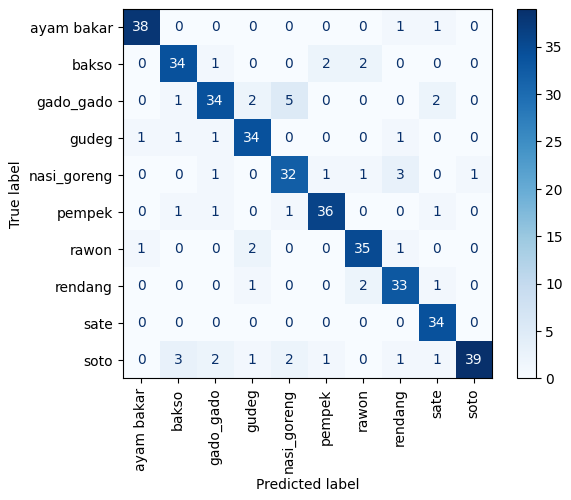
\includegraphics[width=0.9\textwidth, center]{images/confussion-matrix-dgx.png}
    \caption{Visualisasi Confusion Matrix Model mesin DGX A100 Universitas Gunadarma}
    \label{fig:confussion-matrix-dgx}
\end{afigure}

Confusion matrix ini menunjukkan hasil dari model klasifikasi yang telah diuji dengan beberapa kategori makanan Indonesia. Berikut adalah interpretasi dari setiap elemen dalam \textit{confusion matrix} ini:
\begin{itemize}
    \item \textit{True label} (label sebenarnya) berada pada sumbu Y (vertikal).
    \item \textit{Predicted label} (label prediksi) berada pada sumbu X (horizontal).
\end{itemize}

Setiap sel dalam matriks menunjukkan jumlah instance yang diprediksi dalam kategori tertentu. Misalnya, sel pada baris "ayam bakar" dan kolom "ayam bakar" menunjukkan jumlah instance "ayam bakar" yang diprediksi benar oleh model. Berikut adalah beberapa poin penting yang dapat diperhatikan dari \textit{confusion matrix} pada Gambar 4.13:
\begin{itemize}
    \item \textbf{Ayam Bakar}: Dari 40 instance "ayam bakar", 38 diprediksi benar sebagai "ayam bakar", 1 diprediksi sebagai "gudeg", dan 1 diprediksi sebagai "rawon".
    \item \textbf{Bakso}: Dari 40 instance "bakso", 34 diprediksi benar sebagai "bakso", 1 diprediksi sebagai "nasi goreng", 1 diprediksi sebagai "gado-gado", 1 diprediksi sebagai "gudeg", dan 3 diprediksi sebagai "soto".
    \item \textbf{Gado-gado}: Dari 40 instance "gado-gado", 34 diprediksi benar sebagai "gado-gado", 1 diprediksi sebagai "bakso", 1 diprediksi sebagai "gudeg", 1 diprediksi sebagai "nasi goreng", 1 diprediksi sebagai "pempek", dan 2 diprediksi sebagai "soto".
    \item \textbf{Gudeg}: Dari 40 instance "gudeg", 34 diprediksi benar sebagai "gudeg", 2 diprediksi sebagai "gado-gado", 2 diprediksi sebagai "rawon", 1 diprediksi sebagai "rendang", dan 1 diprediksi sebagai "soto".
    \item \textbf{Nasi Goreng}: Dari 40 instance "nasi goreng", 32 diprediksi benar sebagai "nasi goreng", 5 diprediksi sebagai "gado-gado", 1 diprediksi sebagai "pempek", dan 2 diprediksi sebagai "soto".
    \item \textbf{Pempek}: Dari 40 instance "pempek", 36 diprediksi benar sebagai "pempek", 2 diprediksi sebagai "bakso", 1 diprediksi sebagai "nasi goreng", dan 1 diprediksi sebagai "soto".
    \item \textbf{Rawon}: Dari 40 instance "rawon", 35 diprediksi benar sebagai "rawon", 2 diprediksi sebagai "bakso", 1 diprediksi sebagai "nasi goreng", dan 2 diprediksi sebagai "rendang".
    \item \textbf{Rendang}: Dari 40 instance "rendang", 33 diprediksi benar sebagai "rendang", 1 diprediksi sebagai "ayam bakar", 1 diprediksi sebagai "gudeg", 3 diprediksi sebagai "nasi goreng", 1 diprediksi sebagai "rawon", dan 1 diprediksi sebagai "soto".
    \item \textbf{Sate}: Dari 40 instance "sate", 34 diprediksi benar sebagai "sate", 1 diprediksi sebagai "ayam bakar", 2 diprediksi sebagai "gado-gado", 1 diprediksi sebagai "pempek", 1 diprediksi sebagai "rendang", dan 1 diprediksi sebagai "soto".
    \item \textbf{Soto}: Dari 40 instance "soto", 39 diprediksi benar sebagai "soto", 1 diprediksi sebagai "nasi goreng".
\end{itemize}

Secara keseluruhan, model menunjukkan performa yang cukup baik dengan sebagian besar prediksi berada di diagonal utama, yang berarti banyak instance yang diklasifikasikan dengan benar. Namun, ada beberapa kesalahan prediksi yang perlu diperhatikan untuk meningkatkan akurasi model lebih lanjut.

\subsubsection{Hasil Visualisasi Grad-CAM}
Setelah melakukan proses Evaluasi Model, selanjutnya dilakukan proses Visualisasi Grad-CAM. Hal ini dilakukan untuk mengetahui bagaimana model melihat citra dan area mana yang dianggap penting oleh model dalam membuat prediksi. Berikut hasil visualisasi menggunakan Grad-CAM:

\begin{afigure}
    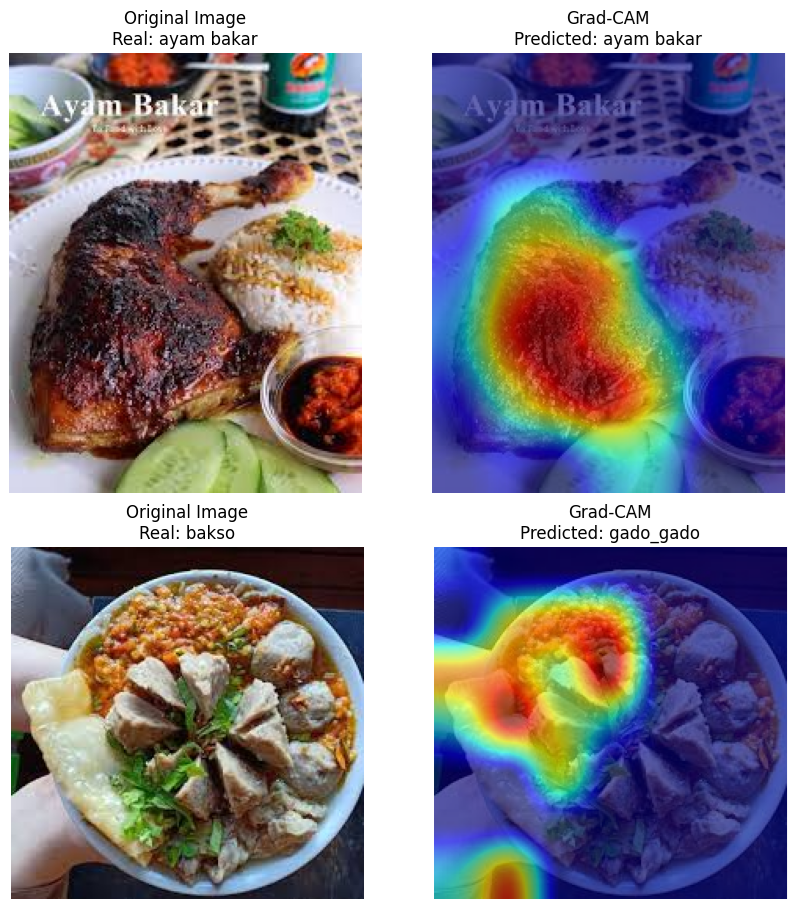
\includegraphics[width=0.9\textwidth, center]{images/grad-cam-1-dgx.png}
    \label{fig:grad-cam-1-dgx}
\end{afigure}
\clearpage
\begin{afigure}
    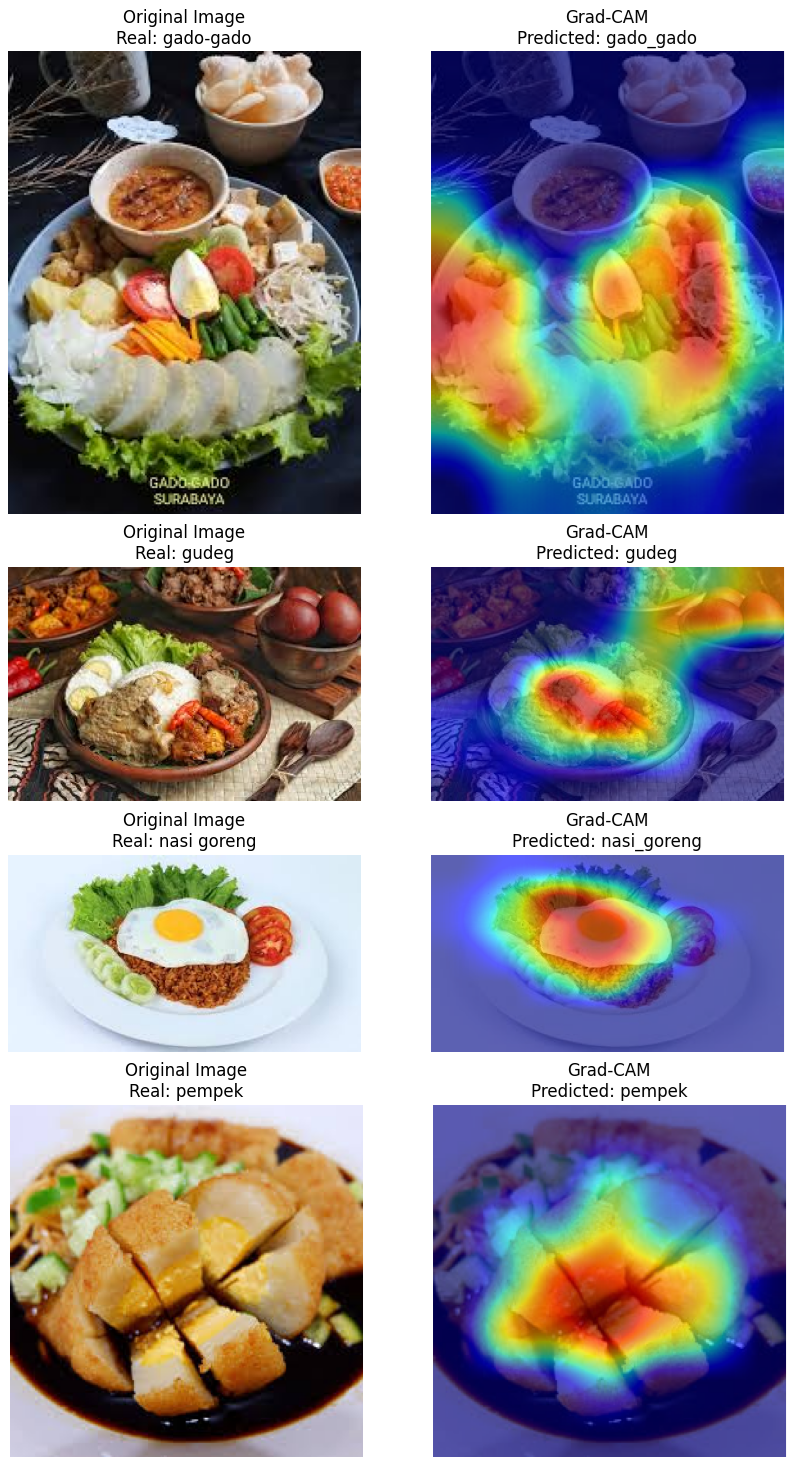
\includegraphics[height=0.9\textheight, width=0.9\textwidth, center]{images/grad-cam-2-dgx.png}
    \label{fig:grad-cam-2-dgx}
\end{afigure}
\clearpage
\begin{afigure}
    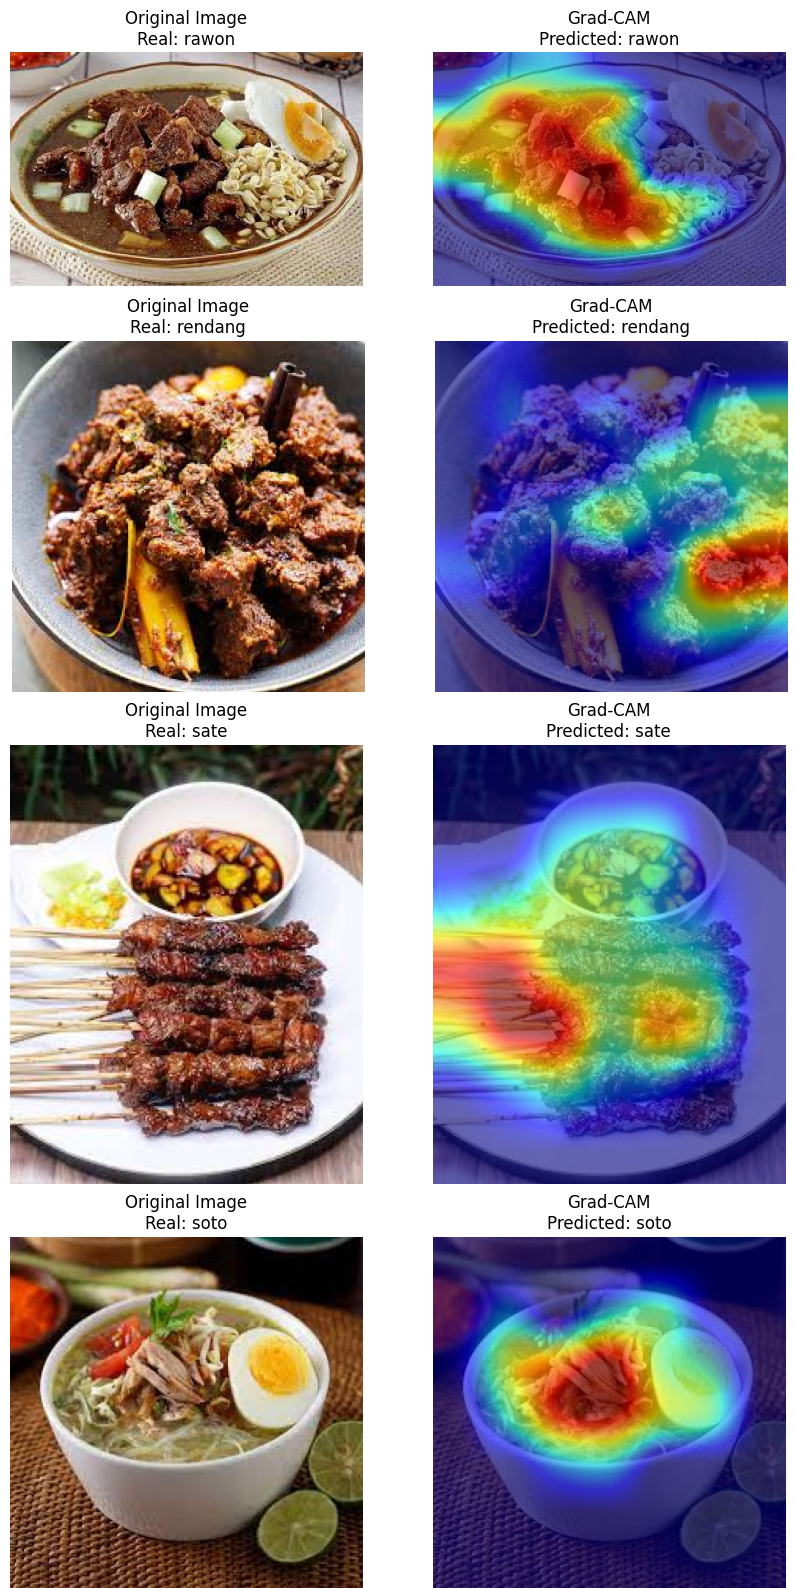
\includegraphics[height=0.9\textheight, width=0.9\textwidth, center]{images/grad-cam-3-dgx.png}
    \caption{Hasil Visualisasi Grad-CAM Model mesin DGX A100 Universitas Gunadarma}
    \label{fig:grad-cam-3-dgx}
\end{afigure}
\clearpage

Pada Gambar 4.14, terlihat bahwa model mampu mengklasifikasikan 9 dari 10 citra dengan tepat. Namun, terdapat satu kelas yang memerlukan perhatian lebih lanjut, yaitu kelas bakso. Dalam visualisasi tersebut, kelas bakso diklasifikasikan sebagai gado-gado. Hal ini menunjukkan bahwa model mengalami kesulitan dalam membedakan antara kedua jenis makanan tersebut.

\subsubsection{Hasil Pengujian Model menggunakan data nutrisi makanan}
Setelah memastikan model memiliki performa yang bagus, selanjutnya dilakukan uji coba menggunakan data nutrisi makanan. Makanan yang berhasil diklasifikasikan kemudian akan ditampilkan informasi nutrisi pada makanan tersebut. Berikut hasil dari uji coba model menggunakan data nutrisi makanan: 
\begin{afigure}
    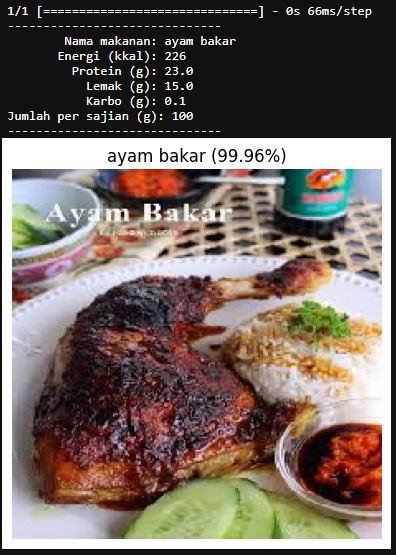
\includegraphics[height=0.55\textheight, width=0.9\textwidth, center]{images/predict-1-dgx.png}
    \label{fig:predict-1-dgx}
\end{afigure}
\pagebreak
\begin{afigure}
    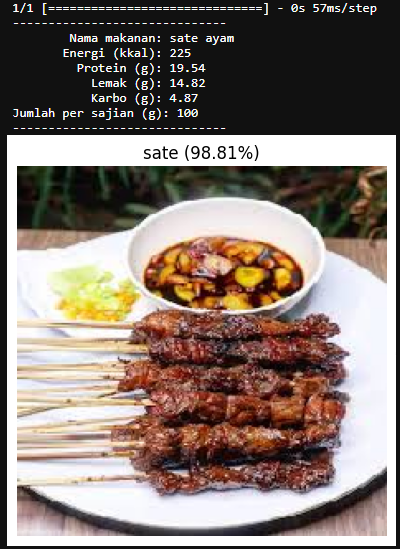
\includegraphics[height=0.55\textheight, width=0.9\textwidth, center]{images/predict-2-dgx.png}
    \caption{Hasil Pengujian Model mesin DGX A100 Universitas Gunadarma menggunakan data nutrisi makanan}
    \label{fig:predict-2-dgx}
\end{afigure}

Pada Gambar 4.15 terlihat bahwa model dapat digunakan dan informasi nutrisi dapat ditampilkan dengan baik. Citra juga berhasil diklasifikasikan dengan tepat, citra pertama berhasil diklasifikasikan sebagai ayam bakar dengan \textit{confidence} sebesar 99.96\%, kemudian citra kedua berhasil diklasifikasikan sebagai sate dengan \textit{confidence} sebesar 98.81\%.




















    \chapter{PENUTUP}

\section{Kesimpulan}
Berdasarkan hasil penelitian yang telah dilakukan untuk identifikasi nilai nutrisi pada makanan populer di Indonesia berbasis citra menggunakan \textit{Convolutional Neural Networ}k (CNN) dengan arsitektur EfficientNetV2, dapat disimpulkan bahwa:
\begin{enumerate}
    \item Model \textit{deep learning} berbasis arsitektur EfficientNetV2 berhasil mengklasifikasikan citra makanan dan menampilkan estimasi nilai nutrisinya.
    \item Model \textit{deep learning} berbasis arsitektur EfficientNetV2 menggunakan Google Colab dengan GPU T4 berhasil mendapatkan nilai \textit{accuracy} sebesar 91,12\% pada data latih dan berhasil mendapatkan nilai \textit{accuracy} sebesar 87,50\% pada data validasi, model juga memiliki rata-rata \textit{precision}, \textit{recall}, dan \textit{F1-Score} sebesar 88\%. Kemudian pengujian model menggunakan DGX A100 berhasil mendapatkan nilai \textit{accuracy} sebesar 91,62\% pada data latih dan berhasil mendapatkan nilai \textit{accuracy} sebesar 87,25\% pada data validasi, model juga memiliki rata-rata \textit{precision} sebesar 87\%, \textit{recall} sebesar 88\%, dan \textit{F1-Score} sebesar 87\%.
    \item Mesin DGX A100 terbukti dapat melakukan pelatihan model 2x lebih cepat dari Google Colab dengan GPU T4 pada dataset penelitian ini. Model yang dilatih menggunakan Google Colab dengan GPU T4 dengan model yang dilatih menggunakan DGX A100 mempunyai performa dan akurasi yang hampir sama dan tidak berbeda secara signifikan.
\end{enumerate}

\section{Saran}
Saran yang dapat diberikan pada penelitian berikutnya adalah menggunakan arsitektur CNN selain EfficientNetV2, seperti InceptionV3, ResNet, ataupun arsitektur lainnya. Diharapkan penelitian selanjutnya dapat menggunakan teknik \textit{image recognition} agar dapat mengidentifikasi banyak makanan dalam satu citra sehingga informasi nutrisi makanan lebih akurat. Penelitian ini diharapkan juga dapat dikembangkan lagi untuk diintegrasikan ke aplikasi agar lebih mudah digunakan.

    %-----------------------------------------------------------
    % End Daftar masukan untuk Bab
    %===========================================================

    %===========================================================
    % Daftar Pustaka
    %-----------------------------------------------------------
    \addcontentsline{toc}{chapter}{DAFTAR PUSTAKA}
    \printbibliography[title={DAFTAR PUSTAKA}]
    %-----------------------------------------------------------
    % End Daftar Pustaka
    %===========================================================
    
    %===========================================================
    % Daftar Lampiran
    %-----------------------------------------------------------
    \appendix
    \addcontentsline{toc}{chapter}{LAMPIRAN}
    \addtocontents{toc}{\protect\setcounter{tocdepth}{0}}
    \chapter*{LAMPIRAN}

    %-----------------------------------------------------------
    % End Daftar Lampiran
    %===========================================================
\end{document}